\documentclass[16pt, letterpaper]{article}
\usepackage{amsmath}
\usepackage{amsfonts}
\usepackage{amssymb}
\usepackage{mathtools}
\DeclarePairedDelimiter{\ceil}{\lceil}{\rceil}

\usepackage{algorithm}
\usepackage[noend]{algpseudocode}

\usepackage{tikz}
\usetikzlibrary{positioning,decorations.pathreplacing}

\usepackage{comment}
\usepackage{color,soul}
\setul{0.5ex}{0.5ex}
\setulcolor{red}

\title{Gina Cody School of Computer Science and Software Engineering \\Concordia University
\\COMP 352: Data Structure and Algorithms }
\author{Student: Duc Nguyen}
\date{}

% Add new function for each
\algnewcommand\algorithmicforeach{\textbf{for each}}
\algdef{S}[FOR]{ForEach}[1]{\algorithmicforeach\ #1\ \algorithmicdo}

% Set up treenode drawing
\tikzset{
  treenode/.style = {align=center, inner sep=0pt, text centered,
    font=\sffamily},
  arn_o/.style = {treenode, circle, font=\sffamily\bfseries, draw=black, fill=white, text width=1.7em, dashed}, %  Nodes are being operated
  arn_n/.style = {treenode, circle, white, font=\sffamily\bfseries, draw=black,
    fill=black, text width=1.7em},% Nodes already on the tree
  arn_t/.style = {treenode, circle, black, font=\sffamily\bfseries, draw=black,
    fill=white, text width=1.7em}, % New nodes
  arn_x/.style = {treenode, rectangle, draw=black,
    minimum width=1.0em, minimum height=1.0em}% Empty entry
}

\begin{document}

\begin{titlepage}
\maketitle
\end{titlepage}
\tableofcontents

\section{Draw a Tree statisfies the conditions}
\subsection{Instruction}
Draw a (single) tree T, such that
\begin{itemize}
    \item Each internal node of T stores a single character;
    \item A preorder traversal of T yields: E K D M J G I A C F H B L;
    \item A postorder traversal of T yields: D J I G A M K F L B H C E.
\end{itemize}

\subsection{Tree satisfies the requirements}
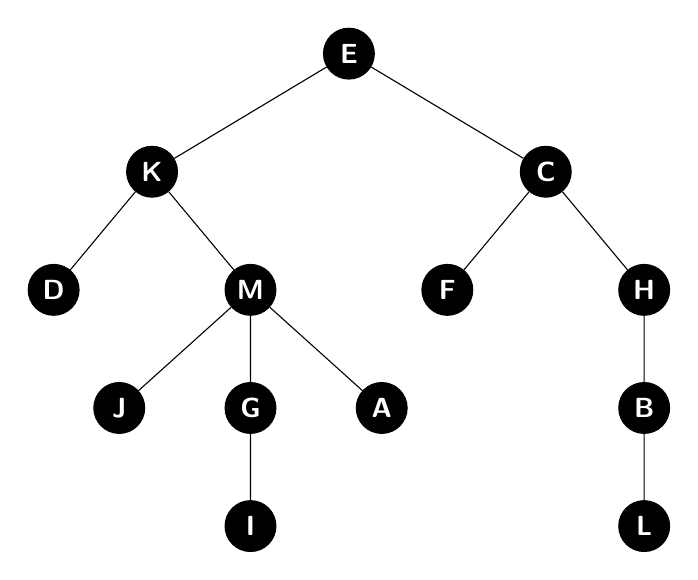
\begin{tikzpicture}[level/.style={sibling distance = 5cm/#1,
  level distance = 1.5cm}] 
\node [arn_n] {E}
    child{ node [arn_n] {K}
        child{ node [arn_n] {D}}
        child{ node [arn_n] {M}
            child{ node [arn_n] {J}}
            child{ node [arn_n] {G}
                child{ node [arn_n] {I}}
                }
            child{ node [arn_n] {A}}
            }
    }
    child{ node [arn_n] {C}
        child{ node [arn_n] {F}}
        child{ node [arn_n] {H}
            child{ node [arn_n] {B}
                child{ node [arn_n] {L}}
            }
        }
    }
;
\end{tikzpicture}
 %-- done
\section{Smallest x numbers in the array}
\subsection{Instruction}
Given an array A of n integers, write an algorithm that finds the smallest x values in the array,
where x $\leq$n. However, the first constraints are given: You are not allowed to use heaps; the array
A should not be modified, and you can only use a maximum auxiliary space of O(n). 

\subsection{Find x smallest elements in the array}
\begin{algorithm}[H]
\caption{Find, and return the x smallest elements in a given array}
\textbf{Input:} the array of integer A, and an integer x represents the requested number of return elements.
\\
\textbf{Output:} x smallest elements from the array A
\begin{algorithmic}[1]
\Procedure{smallestElements}{integer array A, integer x}
\State P $\leftarrow$ priority queue with comparator for integer
\ForEach{value \textbf{v} $\in$ \textbf{A}}
\State P.insert(v)
\EndFor

\State result $\leftarrow$ an integer array to store the result
\State i $\leftarrow$ 0
\While{i $<$ x}
\State result[i] $\leftarrow$ P.removeMin()
\EndWhile
\State \Return result
\EndProcedure
\end{algorithmic}
\end{algorithm}

\textit{Since the algorithm only relies on one more priority queue which has the same number of element as the given array's, the space complexity would be of \textbf{O(n)}.}


 %-- done
\section{Construct a min-heap by bottom-up heap algorithm}
\subsection{Instruction}
Draw the min-heap that results from running the bottom-up heap construction algorithm on the
following list of values:
\\
\begin{center}
\textbf{42 25 49 18 57 105 112 35 38 64 53 20 25 19 16}
\end{center}
Starting from the bottom layer, use the values from left to right as specified above. Show
intermediate steps and the final tree representing the min-heap. Afterwards perform the operation
removeMin() 3 times and show the resulting min-heap after each step.

\subsection{Steps to use bottom-up heap algorithm to construct a min-heap}
\begin{itemize}
    \item There are 15 entries need to be inserted
    \item Therefore, need to construct a heap with height 
    \begin{equation}
        \ceil[\bigg]{\log{(N+1)} - 1}
        = \ceil[\bigg]{\log{(15+1)} - 1} = 3
    \end{equation}
\end{itemize}

\begin{tikzpicture}[level/.style={sibling distance = 5cm/#1,
  level distance = 1.5cm}] 
  \node [arn_x] {}
   child{ node [arn_x] {}
    child{ node [arn_x] {}
        child{ node [arn_x] {}}
        child{ node [arn_x] {}}
    }
    child{ node [arn_x] {}
        child{ node [arn_x] {}}
        child{ node [arn_x] {}}
    }
    }
   child{ node [arn_x] {}
    child{ node [arn_x] {}
        child{ node [arn_x] {}}
        child{ node [arn_x] {}}
    }
    child{ node [arn_x] {}
        child{ node [arn_x] {}}
        child{ node [arn_x] {}}
    }
   }
;
\end{tikzpicture}
\\
\\
\textbf{Initialize Structure (height = 3) with empty entries}
\\
\\

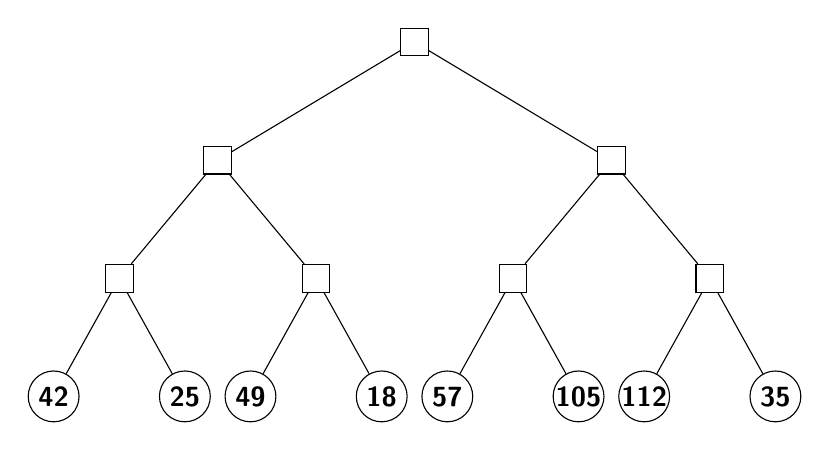
\begin{tikzpicture}[level/.style={sibling distance = 5cm/#1,
  level distance = 1.5cm}] 
  \node [arn_x] {}
   child{ node [arn_x] {}
    child{ node [arn_x] {}
        child{ node [arn_t] {42}}
        child{ node [arn_t] {25}}
    }
    child{ node [arn_x] {}
        child{ node [arn_t] {49}}
        child{ node [arn_t] {18}}
    }
    }
   child{ node [arn_x] {}
    child{ node [arn_x] {}
        child{ node [arn_t] {57}}
        child{ node [arn_t] {105}}
    }
    child{ node [arn_x] {}
        child{ node [arn_t] {112}}
        child{ node [arn_t] {35}}
    }
   }
;
\end{tikzpicture}
\\
\\
\textbf{Construct $\frac{(n+1)}{2} = 8$ first elements to store in each entries at height 3. No bubbling needed}
\\
\\

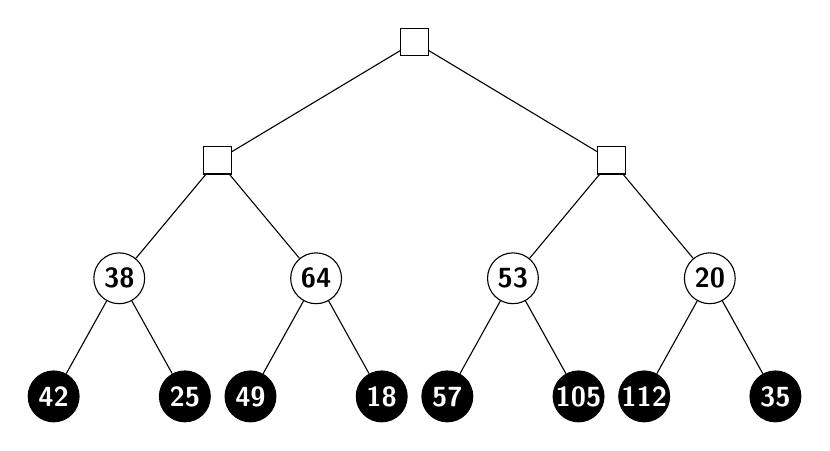
\begin{tikzpicture}[level/.style={sibling distance = 5cm/#1,
  level distance = 1.5cm}] 
  \node [arn_x] {}
   child{ node [arn_x] {}
    child{ node [arn_t] {38}
        child{ node [arn_n] {42}}
        child{ node [arn_n] {25}}
    }
    child{ node [arn_t] {64}
        child{ node [arn_n] {49}}
        child{ node [arn_n] {18}}
    }
    }
   child{ node [arn_x] {}
    child{ node [arn_t] {53}
        child{ node [arn_n] {57}}
        child{ node [arn_n] {105}}
    }
    child{ node [arn_t] {20}
        child{ node [arn_n] {112}}
        child{ node [arn_n] {35}}
    }
   }
;
\end{tikzpicture}
\\
\\
\textbf{Construct $\frac{(n+1)}{4} = 4$ next elements to store in each entries at height 2. Bubbling needed.}
\\
\\

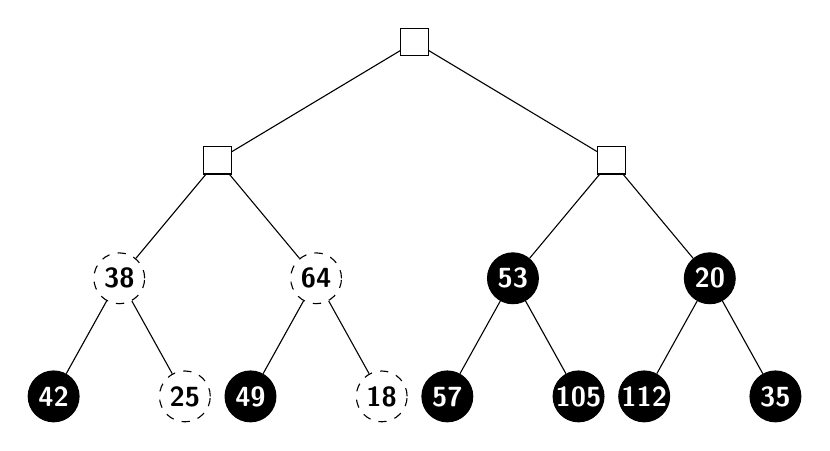
\begin{tikzpicture}[level/.style={sibling distance = 5cm/#1,
  level distance = 1.5cm}] 
  \node [arn_x] {}
   child{ node [arn_x] {}
    child{ node [arn_o] {38}
        child{ node [arn_n] {42}}
        child{ node [arn_o] {25}}
    }
    child{ node [arn_o] {64}
        child{ node [arn_n] {49}}
        child{ node [arn_o] {18}}
    }
    }
   child{ node [arn_x] {}
    child{ node [arn_n] {53}
        child{ node [arn_n] {57}}
        child{ node [arn_n] {105}}
    }
    child{ node [arn_n] {20}
        child{ node [arn_n] {112}}
        child{ node [arn_n] {35}}
    }
   }
;
\end{tikzpicture}
\\
\\
\textbf{Bubbling needed for 38-25 and 64-18.}
\\
\\

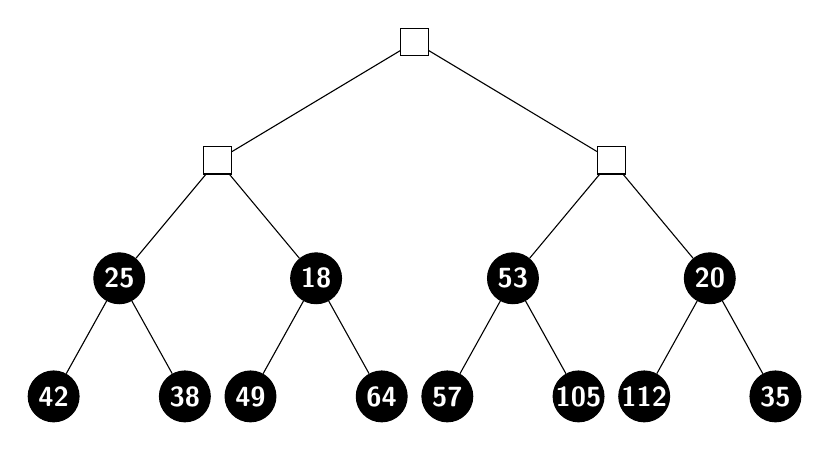
\begin{tikzpicture}[level/.style={sibling distance = 5cm/#1,
  level distance = 1.5cm}] 
  \node [arn_x] {}
   child{ node [arn_x] {}
    child{ node [arn_n] {25}
        child{ node [arn_n] {42}}
        child{ node [arn_n] {38}}
    }
    child{ node [arn_n] {18}
        child{ node [arn_n] {49}}
        child{ node [arn_n] {64}}
    }
    }
   child{ node [arn_x] {}
    child{ node [arn_n] {53}
        child{ node [arn_n] {57}}
        child{ node [arn_n] {105}}
    }
    child{ node [arn_n] {20}
        child{ node [arn_n] {112}}
        child{ node [arn_n] {35}}
    }
   }
;
\end{tikzpicture}
\\
\\
\textbf{Finished bubbling.}
\\
\\

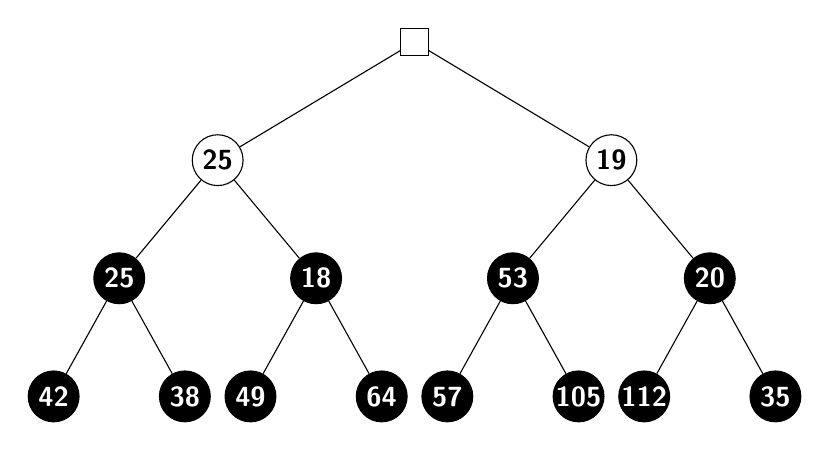
\begin{tikzpicture}[level/.style={sibling distance = 5cm/#1,
  level distance = 1.5cm}] 
  \node [arn_x] {}
   child{ node [arn_t] {25}
    child{ node [arn_n] {25}
        child{ node [arn_n] {42}}
        child{ node [arn_n] {38}}
    }
    child{ node [arn_n] {18}
        child{ node [arn_n] {49}}
        child{ node [arn_n] {64}}
    }
    }
   child{ node [arn_t] {19}
    child{ node [arn_n] {53}
        child{ node [arn_n] {57}}
        child{ node [arn_n] {105}}
    }
    child{ node [arn_n] {20}
        child{ node [arn_n] {112}}
        child{ node [arn_n] {35}}
    }
   }
;
\end{tikzpicture}
\\
\\
\textbf{Construct $\frac{(n+1)}{8} = 2$ next elements to store in each entries at height 1. Bubbling needed.} 
\\
\\

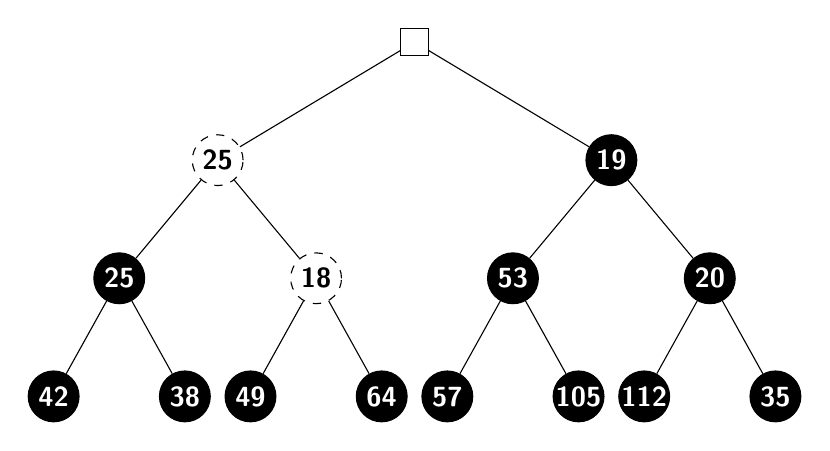
\begin{tikzpicture}[level/.style={sibling distance = 5cm/#1,
  level distance = 1.5cm}] 
  \node [arn_x] {}
   child{ node [arn_o] {25}
    child{ node [arn_n] {25}
        child{ node [arn_n] {42}}
        child{ node [arn_n] {38}}
    }
    child{ node [arn_o] {18}
        child{ node [arn_n] {49}}
        child{ node [arn_n] {64}}
    }
    }
   child{ node [arn_n] {19}
    child{ node [arn_n] {53}
        child{ node [arn_n] {57}}
        child{ node [arn_n] {105}}
    }
    child{ node [arn_n] {20}
        child{ node [arn_n] {112}}
        child{ node [arn_n] {35}}
    }
   }
;
\end{tikzpicture}
\\
\\
\textbf{Bubbling needed for 25-18}
\\
\\

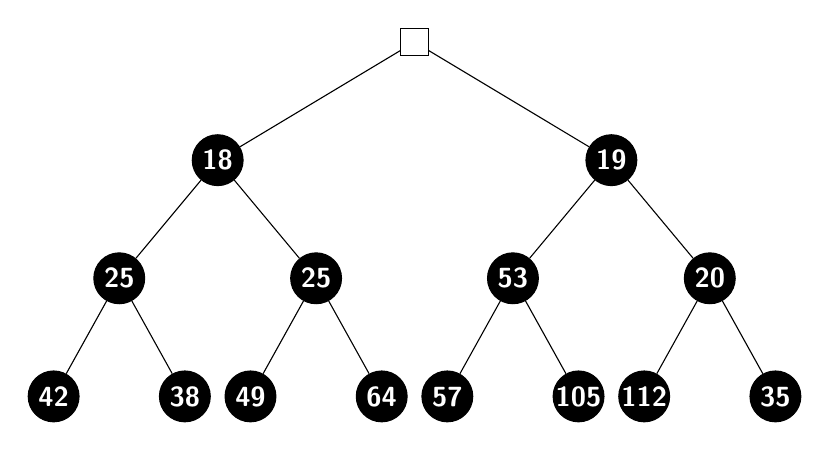
\begin{tikzpicture}[level/.style={sibling distance = 5cm/#1,
  level distance = 1.5cm}] 
  \node [arn_x] {}
   child{ node [arn_n] {18}
    child{ node [arn_n] {25}
        child{ node [arn_n] {42}}
        child{ node [arn_n] {38}}
    }
    child{ node [arn_n] {25}
        child{ node [arn_n] {49}}
        child{ node [arn_n] {64}}
    }
    }
   child{ node [arn_n] {19}
    child{ node [arn_n] {53}
        child{ node [arn_n] {57}}
        child{ node [arn_n] {105}}
    }
    child{ node [arn_n] {20}
        child{ node [arn_n] {112}}
        child{ node [arn_n] {35}}
    }
   }
;
\end{tikzpicture}
\\
\\
\textbf{Finished bubbling.}
\\
\\

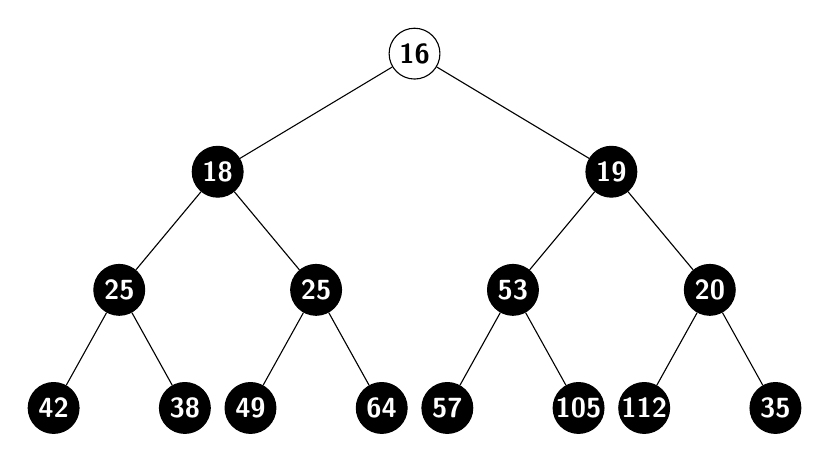
\begin{tikzpicture}[level/.style={sibling distance = 5cm/#1,
  level distance = 1.5cm}] 
  \node [arn_t] {16}
   child{ node [arn_n] {18}
    child{ node [arn_n] {25}
        child{ node [arn_n] {42}}
        child{ node [arn_n] {38}}
    }
    child{ node [arn_n] {25}
        child{ node [arn_n] {49}}
        child{ node [arn_n] {64}}
    }
    }
   child{ node [arn_n] {19}
    child{ node [arn_n] {53}
        child{ node [arn_n] {57}}
        child{ node [arn_n] {105}}
    }
    child{ node [arn_n] {20}
        child{ node [arn_n] {112}}
        child{ node [arn_n] {35}}
    }
   }
;
\end{tikzpicture}
\\
\\
\textbf{Construct $\frac{(n+1)}{16} = 1 $ next element (last element) to store in entry at height 0. No conflict found.} 
\\
\\

\subsection{Final min-heap tree after bottom-up constructing}
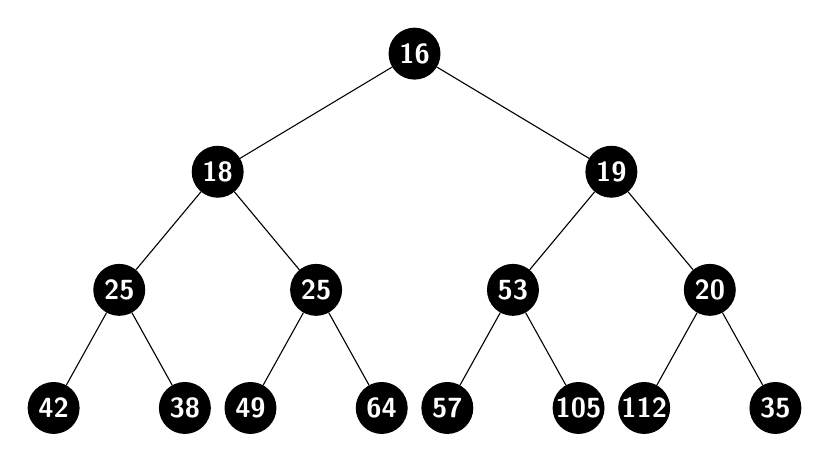
\begin{tikzpicture}[level/.style={sibling distance = 5cm/#1,
  level distance = 1.5cm}] 
  \node [arn_n] {16}
   child{ node [arn_n] {18}
    child{ node [arn_n] {25}
        child{ node [arn_n] {42}}
        child{ node [arn_n] {38}}
    }
    child{ node [arn_n] {25}
        child{ node [arn_n] {49}}
        child{ node [arn_n] {64}}
    }
    }
   child{ node [arn_n] {19}
    child{ node [arn_n] {53}
        child{ node [arn_n] {57}}
        child{ node [arn_n] {105}}
    }
    child{ node [arn_n] {20}
        child{ node [arn_n] {112}}
        child{ node [arn_n] {35}}
    }
   }
;
\end{tikzpicture}

% CALLING REMOVE MIN () 
\subsection{Perform removeMin() 3 times}
\subsubsection{First removeMin()}
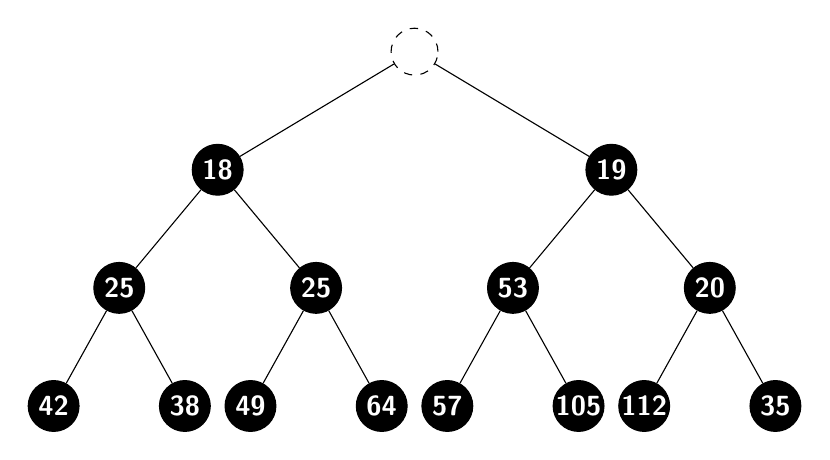
\begin{tikzpicture}[level/.style={sibling distance = 5cm/#1,
  level distance = 1.5cm}] 
  \node [arn_o] {}
   child{ node [arn_n] {18}
    child{ node [arn_n] {25}
        child{ node [arn_n] {42}}
        child{ node [arn_n] {38}}
    }
    child{ node [arn_n] {25}
        child{ node [arn_n] {49}}
        child{ node [arn_n] {64}}
    }
    }
   child{ node [arn_n] {19}
    child{ node [arn_n] {53}
        child{ node [arn_n] {57}}
        child{ node [arn_n] {105}}
    }
    child{ node [arn_n] {20}
        child{ node [arn_n] {112}}
        child{ node [arn_n] {35}}
    }
   }
;
\end{tikzpicture}
\\
\\
\textbf{Remove the root's key. Return the key 16}
\\
\\

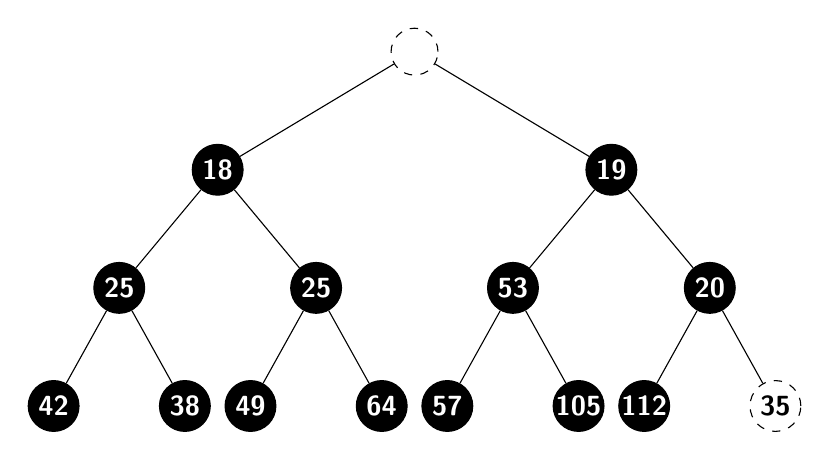
\begin{tikzpicture}[level/.style={sibling distance = 5cm/#1,
  level distance = 1.5cm}] 
  \node [arn_o] {}
   child{ node [arn_n] {18}
    child{ node [arn_n] {25}
        child{ node [arn_n] {42}}
        child{ node [arn_n] {38}}
    }
    child{ node [arn_n] {25}
        child{ node [arn_n] {49}}
        child{ node [arn_n] {64}}
    }
    }
   child{ node [arn_n] {19}
    child{ node [arn_n] {53}
        child{ node [arn_n] {57}}
        child{ node [arn_n] {105}}
    }
    child{ node [arn_n] {20}
        child{ node [arn_n] {112}}
        child{ node [arn_o] {35}}
    }
   }
;
\end{tikzpicture}
\\
\\
\textbf{The last node is 35}
\\
\\

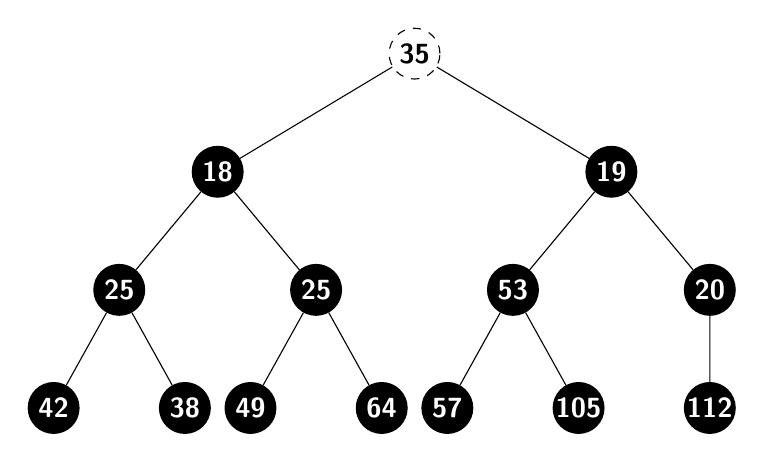
\begin{tikzpicture}[level/.style={sibling distance = 5cm/#1,
  level distance = 1.5cm}] 
  \node [arn_o] {35}
   child{ node [arn_n] {18}
    child{ node [arn_n] {25}
        child{ node [arn_n] {42}}
        child{ node [arn_n] {38}}
    }
    child{ node [arn_n] {25}
        child{ node [arn_n] {49}}
        child{ node [arn_n] {64}}
    }
    }
   child{ node [arn_n] {19}
    child{ node [arn_n] {53}
        child{ node [arn_n] {57}}
        child{ node [arn_n] {105}}
    }
    child{ node [arn_n] {20}
        child{ node [arn_n] {112}}
    }
   }
;
\end{tikzpicture}
\\
\\
\textbf{The entry of the last node will replace the root key. Then, remove the last node out of the heap}
\\
\\

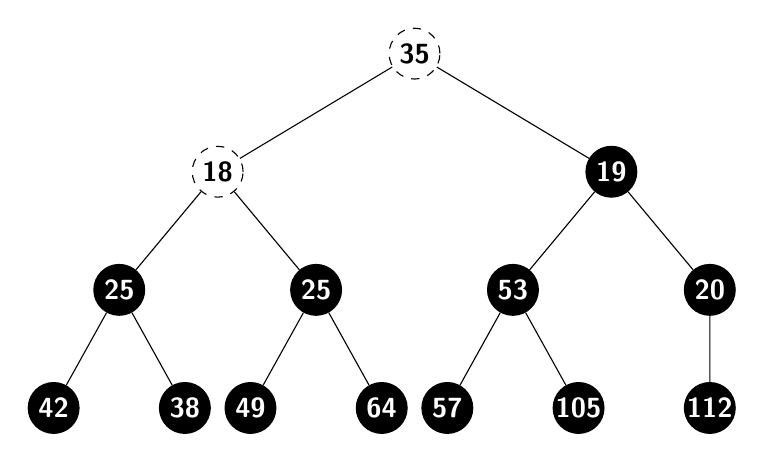
\begin{tikzpicture}[level/.style={sibling distance = 5cm/#1,
  level distance = 1.5cm}] 
  \node [arn_o] {35}
   child{ node [arn_o] {18}
    child{ node [arn_n] {25}
        child{ node [arn_n] {42}}
        child{ node [arn_n] {38}}
    }
    child{ node [arn_n] {25}
        child{ node [arn_n] {49}}
        child{ node [arn_n] {64}}
    }
    }
   child{ node [arn_n] {19}
    child{ node [arn_n] {53}
        child{ node [arn_n] {57}}
        child{ node [arn_n] {105}}
    }
    child{ node [arn_n] {20}
        child{ node [arn_n] {112}}
    }
   }
;
\end{tikzpicture}
\\
\\
\textbf{Start down-heap bubbling for 35-18}
\\
\\

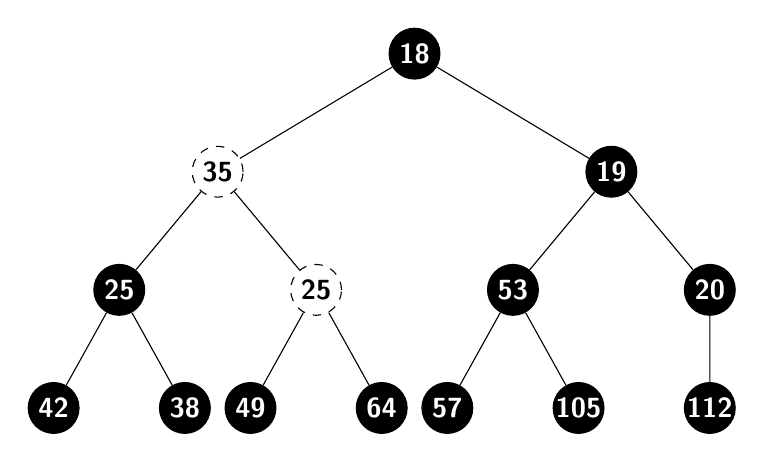
\begin{tikzpicture}[level/.style={sibling distance = 5cm/#1,
  level distance = 1.5cm}] 
  \node [arn_n] {18}
   child{ node [arn_o] {35}
    child{ node [arn_n] {25}
        child{ node [arn_n] {42}}
        child{ node [arn_n] {38}}
    }
    child{ node [arn_o] {25}
        child{ node [arn_n] {49}}
        child{ node [arn_n] {64}}
    }
    }
   child{ node [arn_n] {19}
    child{ node [arn_n] {53}
        child{ node [arn_n] {57}}
        child{ node [arn_n] {105}}
    }
    child{ node [arn_n] {20}
        child{ node [arn_n] {112}}
    }
   }
;
\end{tikzpicture}
\\
\\
\textbf{Continue down-heap bubbling for 35-25}
\\
\\

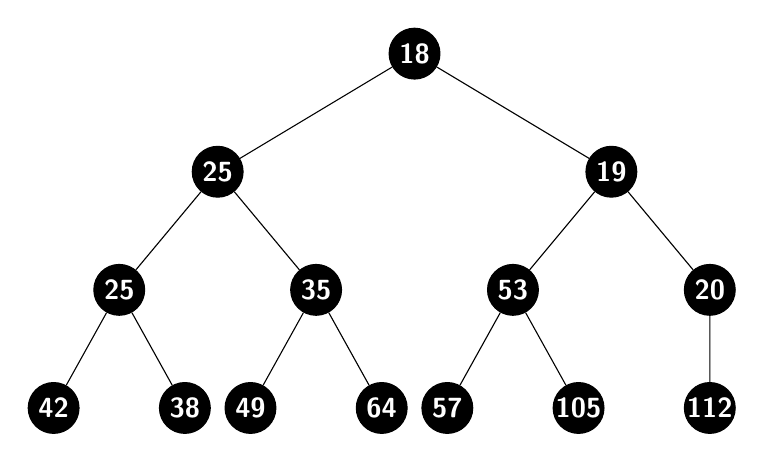
\begin{tikzpicture}[level/.style={sibling distance = 5cm/#1,
  level distance = 1.5cm}] 
  \node [arn_n] {18}
   child{ node [arn_n] {25}
    child{ node [arn_n] {25}
        child{ node [arn_n] {42}}
        child{ node [arn_n] {38}}
    }
    child{ node [arn_n] {35}
        child{ node [arn_n] {49}}
        child{ node [arn_n] {64}}
    }
    }
   child{ node [arn_n] {19}
    child{ node [arn_n] {53}
        child{ node [arn_n] {57}}
        child{ node [arn_n] {105}}
    }
    child{ node [arn_n] {20}
        child{ node [arn_n] {112}}
    }
   }
;
\end{tikzpicture}
\\
\\
\textbf{Finished bubbling}
\\
\\

\subsubsection{Second removeMin()}
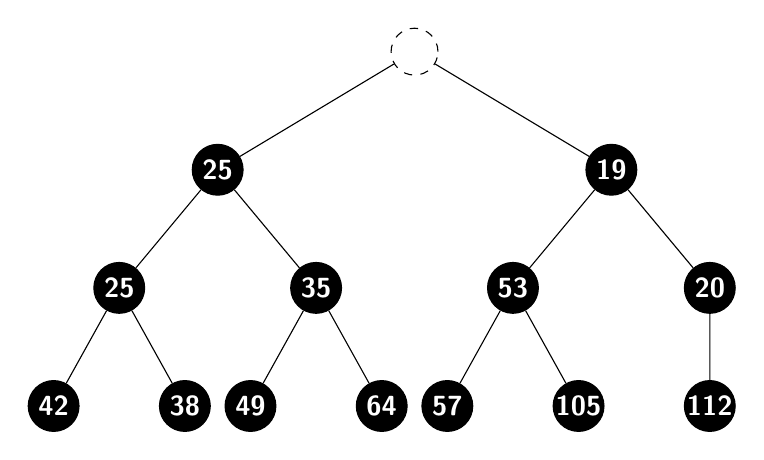
\begin{tikzpicture}[level/.style={sibling distance = 5cm/#1,
  level distance = 1.5cm}] 
  \node [arn_o] {}
   child{ node [arn_n] {25}
    child{ node [arn_n] {25}
        child{ node [arn_n] {42}}
        child{ node [arn_n] {38}}
    }
    child{ node [arn_n] {35}
        child{ node [arn_n] {49}}
        child{ node [arn_n] {64}}
    }
    }
   child{ node [arn_n] {19}
    child{ node [arn_n] {53}
        child{ node [arn_n] {57}}
        child{ node [arn_n] {105}}
    }
    child{ node [arn_n] {20}
        child{ node [arn_n] {112}}
    }
   }
;
\end{tikzpicture}
\\
\\
\textbf{Remove the root's key. Return the key 18}
\\
\\

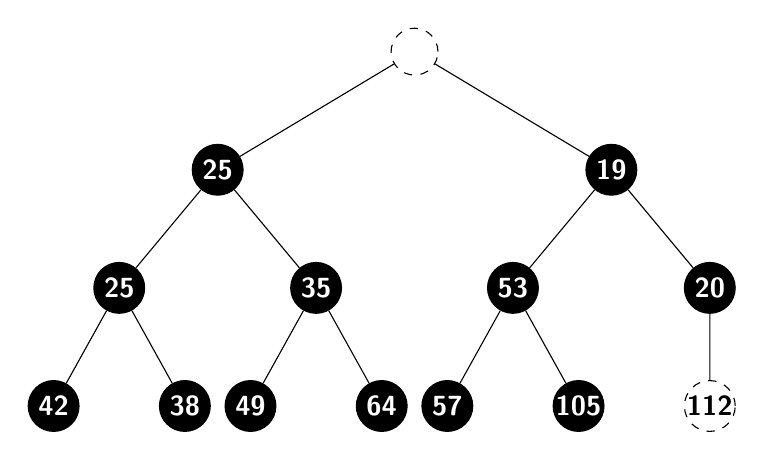
\begin{tikzpicture}[level/.style={sibling distance = 5cm/#1,
  level distance = 1.5cm}] 
  \node [arn_o] {}
   child{ node [arn_n] {25}
    child{ node [arn_n] {25}
        child{ node [arn_n] {42}}
        child{ node [arn_n] {38}}
    }
    child{ node [arn_n] {35}
        child{ node [arn_n] {49}}
        child{ node [arn_n] {64}}
    }
    }
   child{ node [arn_n] {19}
    child{ node [arn_n] {53}
        child{ node [arn_n] {57}}
        child{ node [arn_n] {105}}
    }
    child{ node [arn_n] {20}
        child{ node [arn_o] {112}}
    }
   }
;
\end{tikzpicture}
\\
\\
\textbf{The last node is 112}
\\
\\

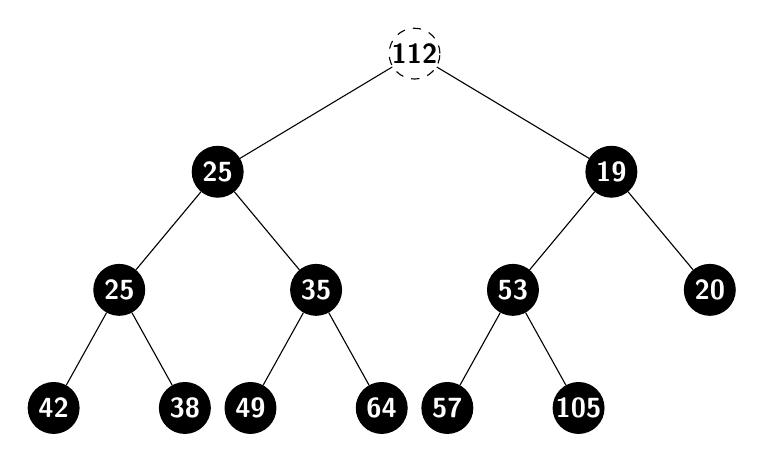
\begin{tikzpicture}[level/.style={sibling distance = 5cm/#1,
  level distance = 1.5cm}] 
  \node [arn_o] {112}
   child{ node [arn_n] {25}
    child{ node [arn_n] {25}
        child{ node [arn_n] {42}}
        child{ node [arn_n] {38}}
    }
    child{ node [arn_n] {35}
        child{ node [arn_n] {49}}
        child{ node [arn_n] {64}}
    }
    }
   child{ node [arn_n] {19}
    child{ node [arn_n] {53}
        child{ node [arn_n] {57}}
        child{ node [arn_n] {105}}
    }
    child{ node [arn_n] {20}}
   }
;
\end{tikzpicture}
\\
\\
\textbf{The entry of the last node will replace the root key. Then, remove the last node out of the heap}
\\
\\

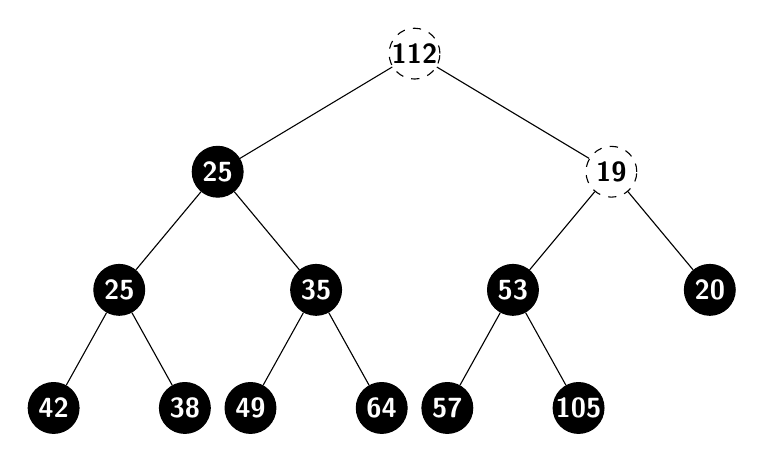
\begin{tikzpicture}[level/.style={sibling distance = 5cm/#1,
  level distance = 1.5cm}] 
  \node [arn_o] {112}
   child{ node [arn_n] {25}
    child{ node [arn_n] {25}
        child{ node [arn_n] {42}}
        child{ node [arn_n] {38}}
    }
    child{ node [arn_n] {35}
        child{ node [arn_n] {49}}
        child{ node [arn_n] {64}}
    }
    }
   child{ node [arn_o] {19}
    child{ node [arn_n] {53}
        child{ node [arn_n] {57}}
        child{ node [arn_n] {105}}
    }
    child{ node [arn_n] {20}}
   }
;
\end{tikzpicture}
\\
\\
\textbf{Start down-heap bubbling for 112-19}
\\
\\

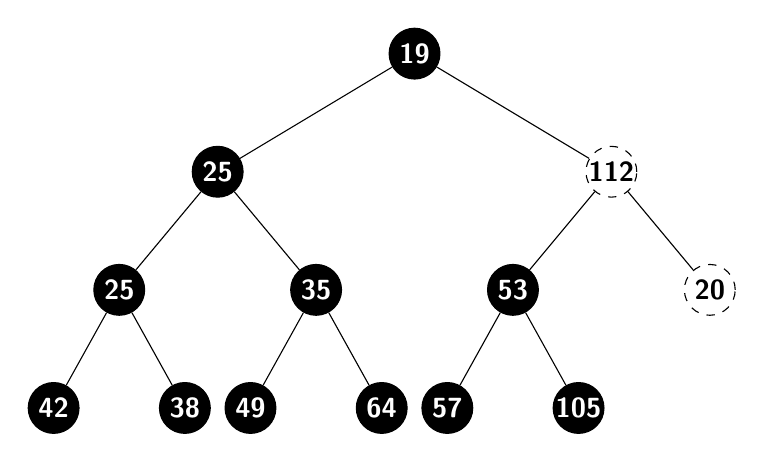
\begin{tikzpicture}[level/.style={sibling distance = 5cm/#1,
  level distance = 1.5cm}] 
  \node [arn_n] {19}
   child{ node [arn_n] {25}
    child{ node [arn_n] {25}
        child{ node [arn_n] {42}}
        child{ node [arn_n] {38}}
    }
    child{ node [arn_n] {35}
        child{ node [arn_n] {49}}
        child{ node [arn_n] {64}}
    }
    }
   child{ node [arn_o] {112}
    child{ node [arn_n] {53}
        child{ node [arn_n] {57}}
        child{ node [arn_n] {105}}
    }
    child{ node [arn_o] {20}}
   }
;
\end{tikzpicture}
\\
\\
\textbf{Continue down-heap bubbling for 112-20}
\\
\\

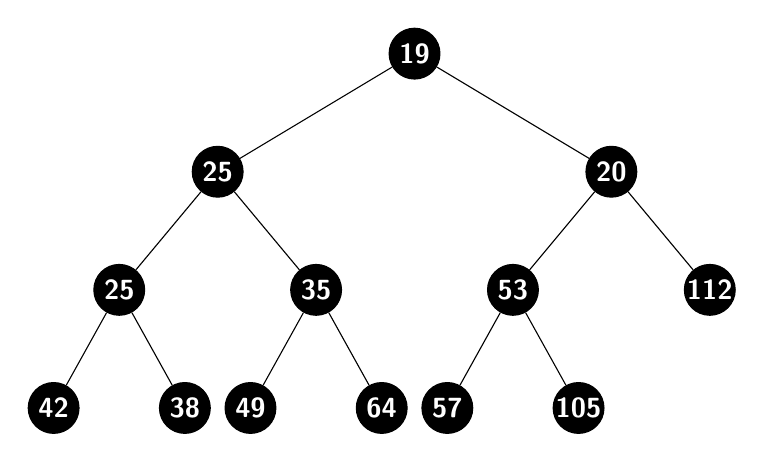
\begin{tikzpicture}[level/.style={sibling distance = 5cm/#1,
  level distance = 1.5cm}] 
  \node [arn_n] {19}
   child{ node [arn_n] {25}
    child{ node [arn_n] {25}
        child{ node [arn_n] {42}}
        child{ node [arn_n] {38}}
    }
    child{ node [arn_n] {35}
        child{ node [arn_n] {49}}
        child{ node [arn_n] {64}}
    }
    }
   child{ node [arn_n] {20}
    child{ node [arn_n] {53}
        child{ node [arn_n] {57}}
        child{ node [arn_n] {105}}
    }
    child{ node [arn_n] {112}}
   }
;
\end{tikzpicture}
\\
\\
\textbf{Finished bubbling}
\\
\\

\subsubsection{Third removeMin()}
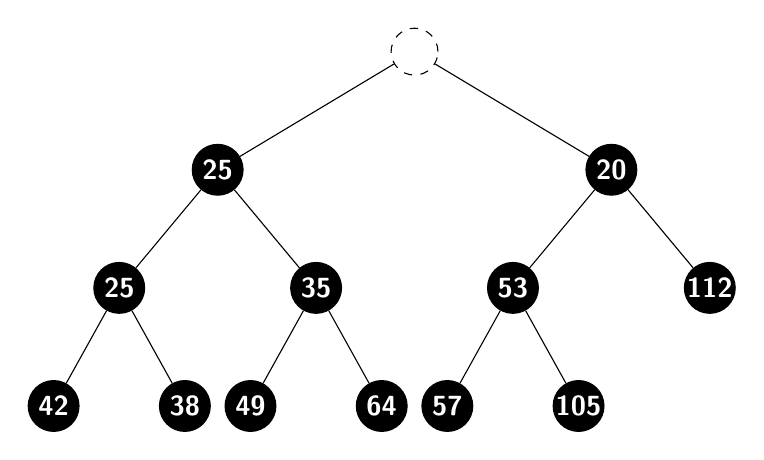
\begin{tikzpicture}[level/.style={sibling distance = 5cm/#1,
  level distance = 1.5cm}] 
  \node [arn_o] {}
   child{ node [arn_n] {25}
    child{ node [arn_n] {25}
        child{ node [arn_n] {42}}
        child{ node [arn_n] {38}}
    }
    child{ node [arn_n] {35}
        child{ node [arn_n] {49}}
        child{ node [arn_n] {64}}
    }
    }
   child{ node [arn_n] {20}
    child{ node [arn_n] {53}
        child{ node [arn_n] {57}}
        child{ node [arn_n] {105}}
    }
    child{ node [arn_n] {112}}
   }
;
\end{tikzpicture}
\\
\\
\textbf{Remove the root's key. Return the key 19}
\\
\\

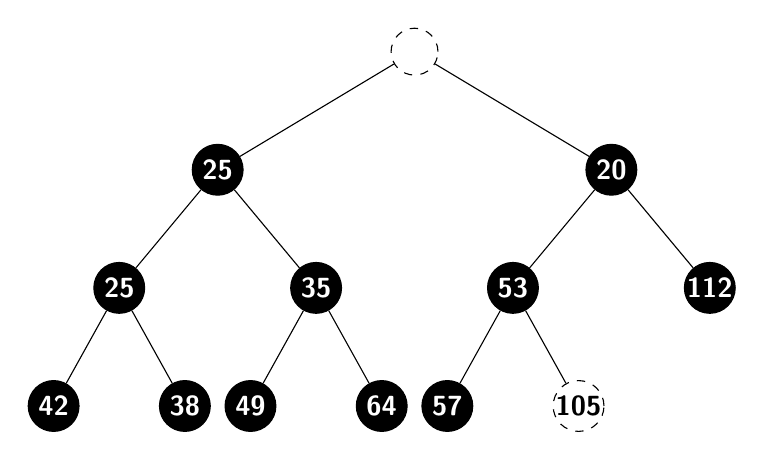
\begin{tikzpicture}[level/.style={sibling distance = 5cm/#1,
  level distance = 1.5cm}] 
  \node [arn_o] {}
   child{ node [arn_n] {25}
    child{ node [arn_n] {25}
        child{ node [arn_n] {42}}
        child{ node [arn_n] {38}}
    }
    child{ node [arn_n] {35}
        child{ node [arn_n] {49}}
        child{ node [arn_n] {64}}
    }
    }
   child{ node [arn_n] {20}
    child{ node [arn_n] {53}
        child{ node [arn_n] {57}}
        child{ node [arn_o] {105}}
    }
    child{ node [arn_n] {112}}
   }
;
\end{tikzpicture}
\\
\\
\textbf{The last node is 105}
\\
\\

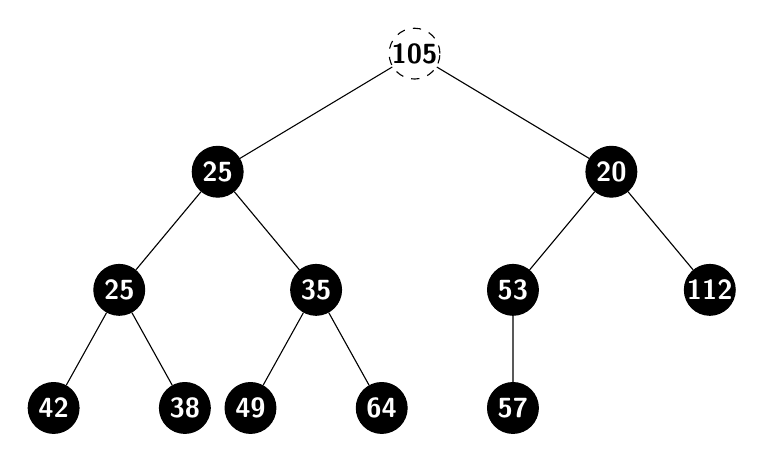
\begin{tikzpicture}[level/.style={sibling distance = 5cm/#1,
  level distance = 1.5cm}] 
  \node [arn_o] {105}
   child{ node [arn_n] {25}
    child{ node [arn_n] {25}
        child{ node [arn_n] {42}}
        child{ node [arn_n] {38}}
    }
    child{ node [arn_n] {35}
        child{ node [arn_n] {49}}
        child{ node [arn_n] {64}}
    }
    }
   child{ node [arn_n] {20}
    child{ node [arn_n] {53}
        child{ node [arn_n] {57}}
    }
    child{ node [arn_n] {112}}
   }
;
\end{tikzpicture}
\\
\\
\textbf{The entry of the last node will replace the root key. Then, remove the last node out of the heap}
\\
\\

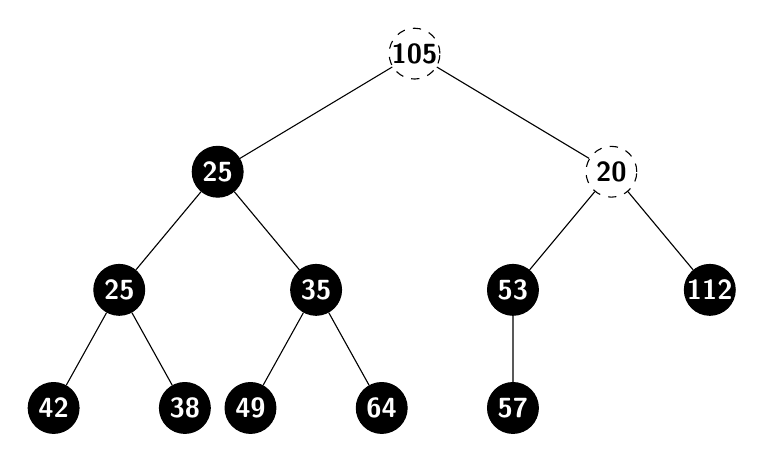
\begin{tikzpicture}[level/.style={sibling distance = 5cm/#1,
  level distance = 1.5cm}] 
  \node [arn_o] {105}
   child{ node [arn_n] {25}
    child{ node [arn_n] {25}
        child{ node [arn_n] {42}}
        child{ node [arn_n] {38}}
    }
    child{ node [arn_n] {35}
        child{ node [arn_n] {49}}
        child{ node [arn_n] {64}}
    }
    }
   child{ node [arn_o] {20}
    child{ node [arn_n] {53}
        child{ node [arn_n] {57}}
    }
    child{ node [arn_n] {112}}
   }
;
\end{tikzpicture}
\\
\\
\textbf{Start down-heap bubbling for 105-20}
\\
\\

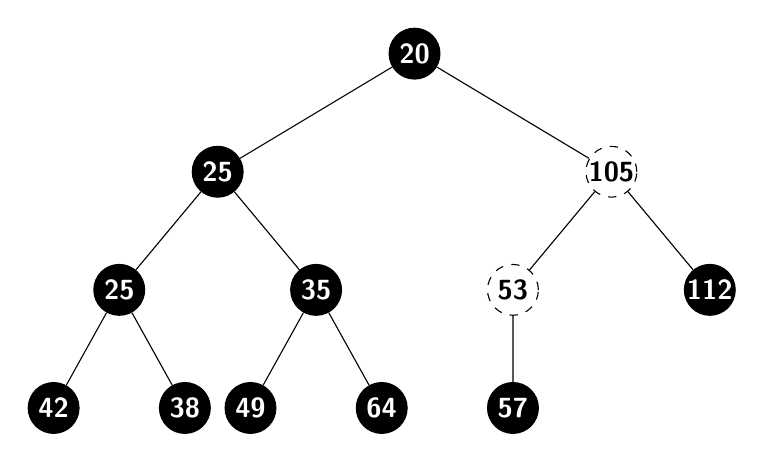
\begin{tikzpicture}[level/.style={sibling distance = 5cm/#1,
  level distance = 1.5cm}] 
  \node [arn_n] {20}
   child{ node [arn_n] {25}
    child{ node [arn_n] {25}
        child{ node [arn_n] {42}}
        child{ node [arn_n] {38}}
    }
    child{ node [arn_n] {35}
        child{ node [arn_n] {49}}
        child{ node [arn_n] {64}}
    }
    }
   child{ node [arn_o] {105}
    child{ node [arn_o] {53}
        child{ node [arn_n] {57}}
    }
    child{ node [arn_n] {112}}
   }
;
\end{tikzpicture}
\\
\\
\textbf{Continue down-heap bubbling for 105-53}
\\
\\

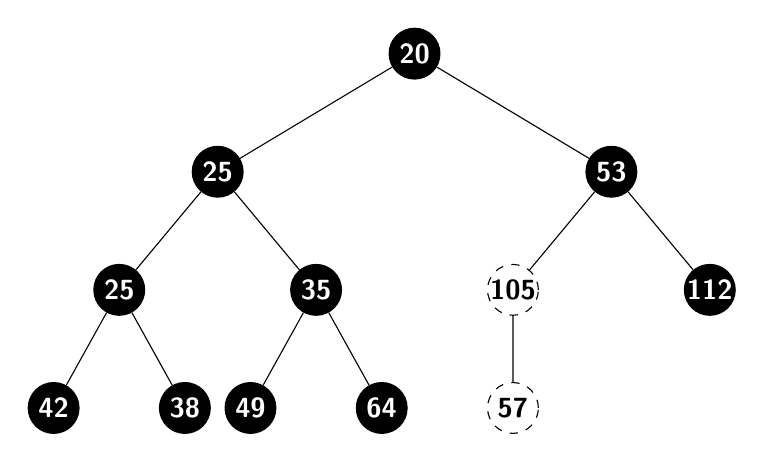
\begin{tikzpicture}[level/.style={sibling distance = 5cm/#1,
  level distance = 1.5cm}] 
  \node [arn_n] {20}
   child{ node [arn_n] {25}
    child{ node [arn_n] {25}
        child{ node [arn_n] {42}}
        child{ node [arn_n] {38}}
    }
    child{ node [arn_n] {35}
        child{ node [arn_n] {49}}
        child{ node [arn_n] {64}}
    }
    }
   child{ node [arn_n] {53}
    child{ node [arn_o] {105}
        child{ node [arn_o] {57}}
    }
    child{ node [arn_n] {112}}
   }
;
\end{tikzpicture}
\\
\\
\textbf{Continue down-heap bubbling for 105-57}
\\
\\

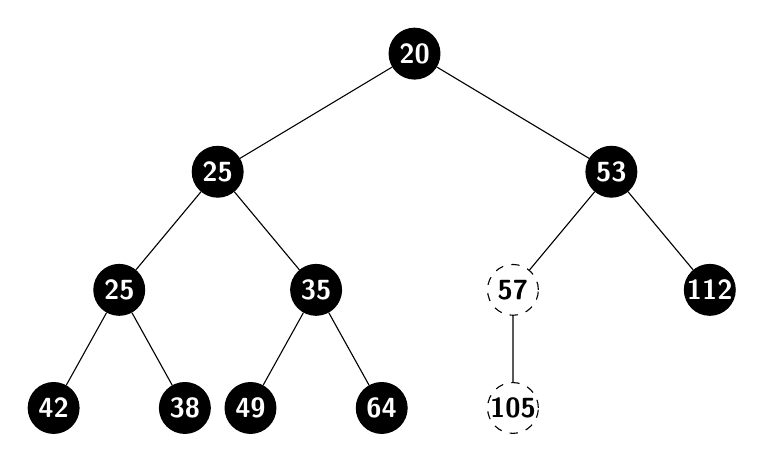
\begin{tikzpicture}[level/.style={sibling distance = 5cm/#1,
  level distance = 1.5cm}] 
  \node [arn_n] {20}
   child{ node [arn_n] {25}
    child{ node [arn_n] {25}
        child{ node [arn_n] {42}}
        child{ node [arn_n] {38}}
    }
    child{ node [arn_n] {35}
        child{ node [arn_n] {49}}
        child{ node [arn_n] {64}}
    }
    }
   child{ node [arn_n] {53}
    child{ node [arn_o] {57}
        child{ node [arn_o] {105}}
    }
    child{ node [arn_n] {112}}
   }
;
\end{tikzpicture}
\\
\\
\textbf{Finished bubbling}
\\
\\

\subsection{Final Min-heap tree}
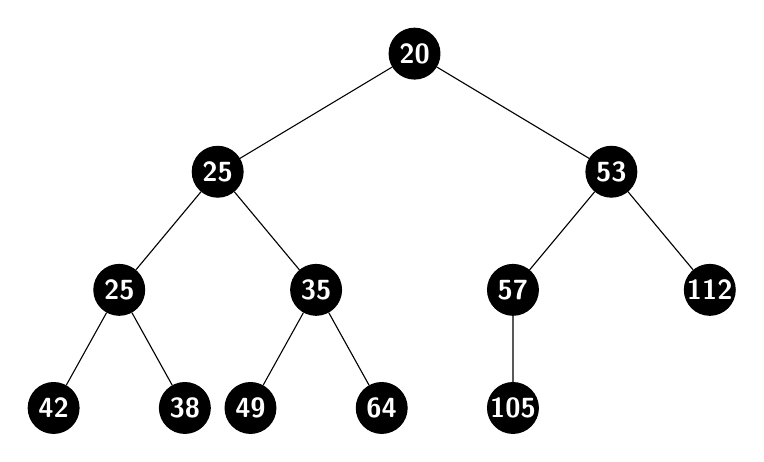
\begin{tikzpicture}[level/.style={sibling distance = 5cm/#1,
  level distance = 1.5cm}] 
  \node [arn_n] {20}
   child{ node [arn_n] {25}
    child{ node [arn_n] {25}
        child{ node [arn_n] {42}}
        child{ node [arn_n] {38}}
    }
    child{ node [arn_n] {35}
        child{ node [arn_n] {49}}
        child{ node [arn_n] {64}}
    }
    }
   child{ node [arn_n] {53}
    child{ node [arn_n] {57}
        child{ node [arn_n] {105}}
    }
    child{ node [arn_n] {112}}
   }
;
\end{tikzpicture} %-- done
\section{Create a max-heap}
\subsection{Instruction}
Create a max-heap using the list of values from Question 3 above but this time you have to insert
these values one by one using the order from left to right (i.e insert 42, then 25, then 49, etc.).
Show the tree after each step and the final tree representing the max-heap.

\subsection{Step-by-step process to construct the Max-heap tree}
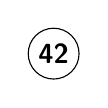
\begin{tikzpicture}[level/.style={sibling distance = 5cm/#1,
  level distance = 1.5cm}] 
  \node [arn_t] {42};
\end{tikzpicture}
\\
\textbf{Adding 42 to the heap}
\\
\\
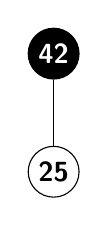
\begin{tikzpicture}[level/.style={sibling distance = 5cm/#1,
  level distance = 1.5cm}] 
  \node [arn_n] {42}
   child{ node [arn_t] {25}}
;
\end{tikzpicture}
\\
\\
\textbf{Adding 25 to the heap. No conflict found}
\\
\\

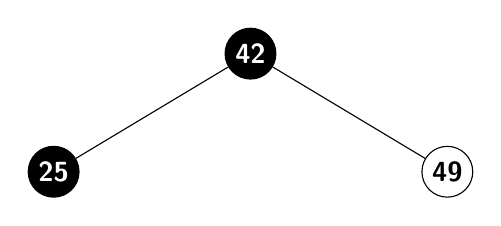
\begin{tikzpicture}[level/.style={sibling distance = 5cm/#1,
  level distance = 1.5cm}] 
  \node [arn_n] {42}
   child{ node [arn_n] {25}}
   child{ node [arn_t] {49}}
;
\end{tikzpicture}
\\
\\
\textbf{Adding 49 to the heap. Conflict found. Bubbling up}
\\
\\

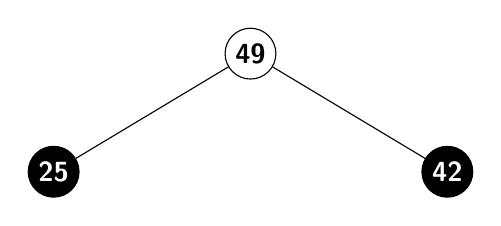
\begin{tikzpicture}[level/.style={sibling distance = 5cm/#1,
  level distance = 1.5cm}] 
  \node [arn_t] {49}
   child{ node [arn_n] {25}}
   child{ node [arn_n] {42}}
;
\end{tikzpicture}
\\
\\
\textbf{Swapping with its parents. $49>42$. No remaining conflict}
\\
\\

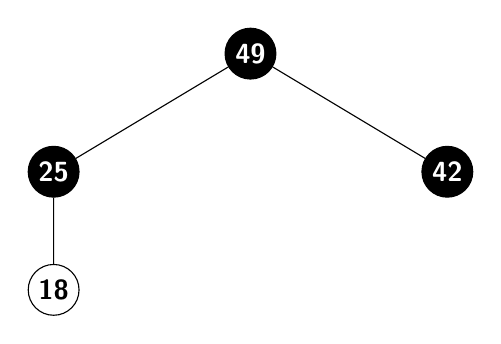
\begin{tikzpicture}[level/.style={sibling distance = 5cm/#1,
  level distance = 1.5cm}] 
  \node [arn_n] {49}
   child{ node [arn_n] {25}
    child{ node [arn_t] {18}}
    }
   child{ node [arn_n] {42}}
;
\end{tikzpicture}
\\
\\
\textbf{Adding 18 to the heap. No conflict found}
\\
\\

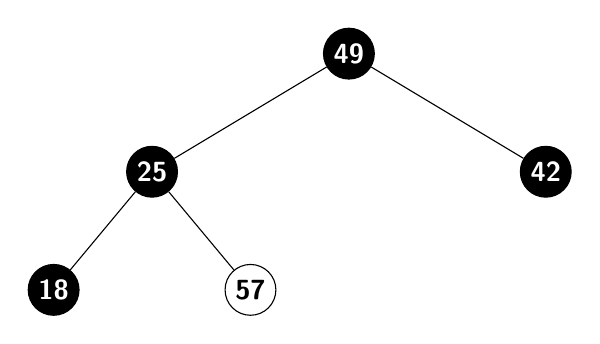
\begin{tikzpicture}[level/.style={sibling distance = 5cm/#1,
  level distance = 1.5cm}] 
  \node [arn_n] {49}
   child{ node [arn_n] {25}
    child{ node [arn_n] {18}}
    child{ node [arn_t] {57}}
    }
   child{ node [arn_n] {42}}
;
\end{tikzpicture}
\\
\\
\textbf{Adding 57 to the heap. Conflict found. Bubbling up}
\\
\\

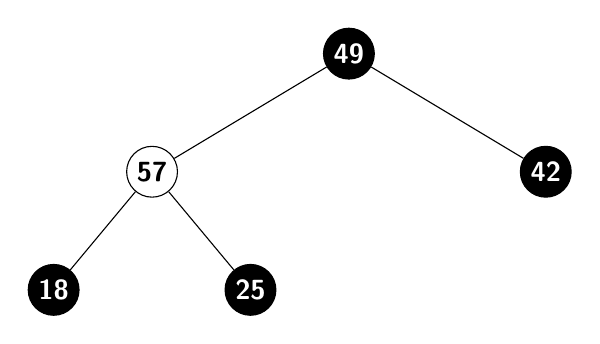
\begin{tikzpicture}[level/.style={sibling distance = 5cm/#1,
  level distance = 1.5cm}] 
  \node [arn_n] {49}
   child{ node [arn_t] {57}
    child{ node [arn_n] {18}}
    child{ node [arn_n] {25}}
    }
   child{ node [arn_n] {42}}
;
\end{tikzpicture}
\\
\\
\textbf{Swapping with its parents. $57>25$. Still having conflict. Continue bubbling up}
\\
\\

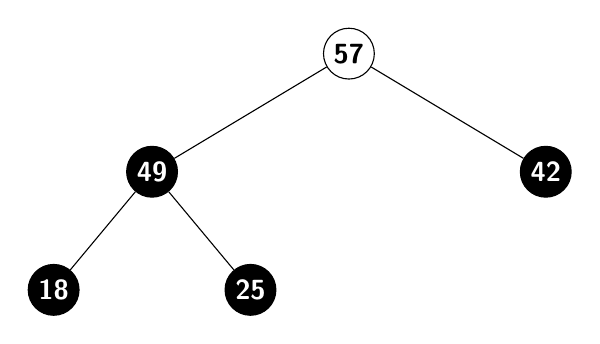
\begin{tikzpicture}[level/.style={sibling distance = 5cm/#1,
  level distance = 1.5cm}] 
  \node [arn_t] {57}
   child{ node [arn_n] {49}
    child{ node [arn_n] {18}}
    child{ node [arn_n] {25}}
    }
   child{ node [arn_n] {42}}
;
\end{tikzpicture}
\\
\\
\textbf{Swapping with its parents. $57>49$. No remaining conflict}
\\
\\

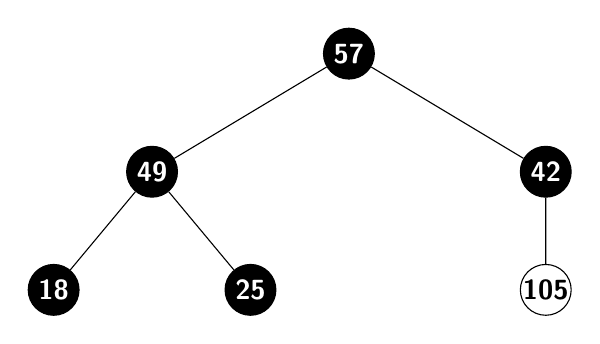
\begin{tikzpicture}[level/.style={sibling distance = 5cm/#1,
  level distance = 1.5cm}] 
  \node [arn_n] {57}
   child{ node [arn_n] {49}
    child{ node [arn_n] {18}}
    child{ node [arn_n] {25}}
    }
   child{ node [arn_n] {42}
    child{ node [arn_t] {105}}
   }
;
\end{tikzpicture}
\\
\\
\textbf{Adding 105 to the heap. Conflict found. Bubbling up}
\\
\\

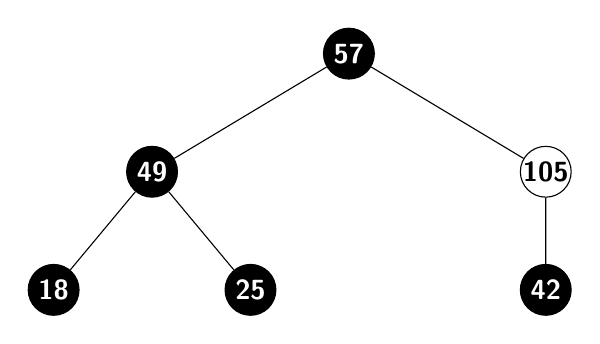
\begin{tikzpicture}[level/.style={sibling distance = 5cm/#1,
  level distance = 1.5cm}] 
  \node [arn_n] {57}
   child{ node [arn_n] {49}
    child{ node [arn_n] {18}}
    child{ node [arn_n] {25}}
    }
   child{ node [arn_t] {105}
    child{ node [arn_n] {42}}
   }
;
\end{tikzpicture}
\\
\\
\textbf{Swapping with its parents. $105>42$. Still having conflict. Continue bubbling up}
\\
\\

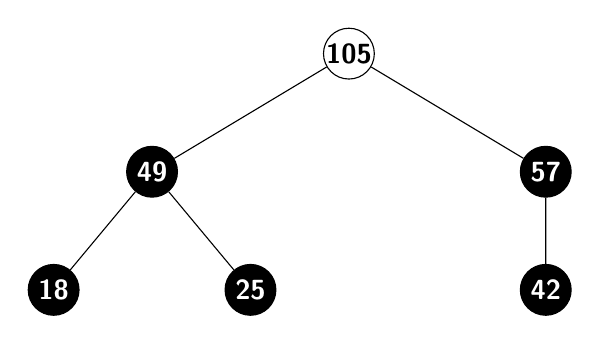
\begin{tikzpicture}[level/.style={sibling distance = 5cm/#1,
  level distance = 1.5cm}] 
  \node [arn_t] {105}
   child{ node [arn_n] {49}
    child{ node [arn_n] {18}}
    child{ node [arn_n] {25}}
    }
   child{ node [arn_n] {57}
    child{ node [arn_n] {42}}
   }
;
\end{tikzpicture}
\\
\\
\textbf{Swapping with its parents. $105>57$. No remaining conflict}
\\
\\

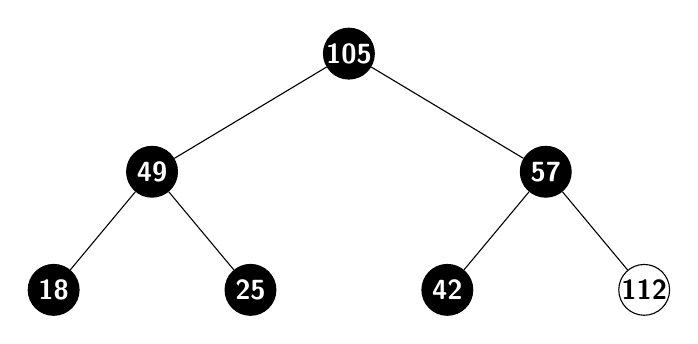
\begin{tikzpicture}[level/.style={sibling distance = 5cm/#1,
  level distance = 1.5cm}] 
  \node [arn_n] {105}
   child{ node [arn_n] {49}
    child{ node [arn_n] {18}}
    child{ node [arn_n] {25}}
    }
   child{ node [arn_n] {57}
    child{ node [arn_n] {42}}
    child{ node [arn_t] {112}}
   }
;
\end{tikzpicture}
\\
\\
\textbf{Adding 112 to the heap. Conflict found. Bubbling up}
\\
\\

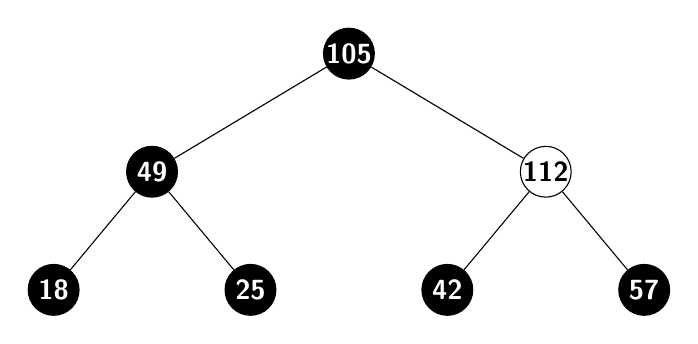
\begin{tikzpicture}[level/.style={sibling distance = 5cm/#1,
  level distance = 1.5cm}] 
  \node [arn_n] {105}
   child{ node [arn_n] {49}
    child{ node [arn_n] {18}}
    child{ node [arn_n] {25}}
    }
   child{ node [arn_t] {112}
    child{ node [arn_n] {42}}
    child{ node [arn_n] {57}}
   }
;
\end{tikzpicture}
\\
\\
\textbf{Swapping with its parents. $112>57$. Still having conflict. Continue bubbling up}
\\
\\

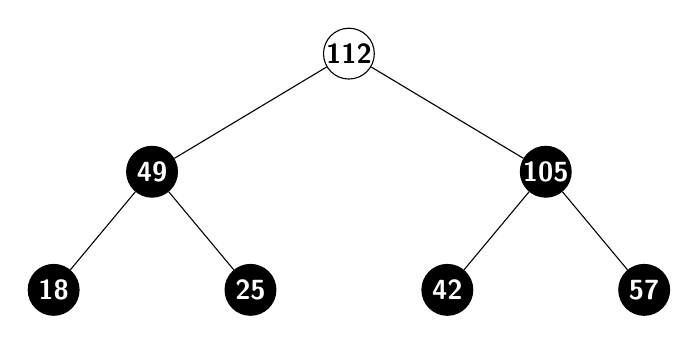
\begin{tikzpicture}[level/.style={sibling distance = 5cm/#1,
  level distance = 1.5cm}] 
  \node [arn_t] {112}
   child{ node [arn_n] {49}
    child{ node [arn_n] {18}}
    child{ node [arn_n] {25}}
    }
   child{ node [arn_n] {105}
    child{ node [arn_n] {42}}
    child{ node [arn_n] {57}}
   }
;
\end{tikzpicture}
\\
\\
\textbf{Swapping with its parents. $112>105$. No remaining conflict}
\\
\\

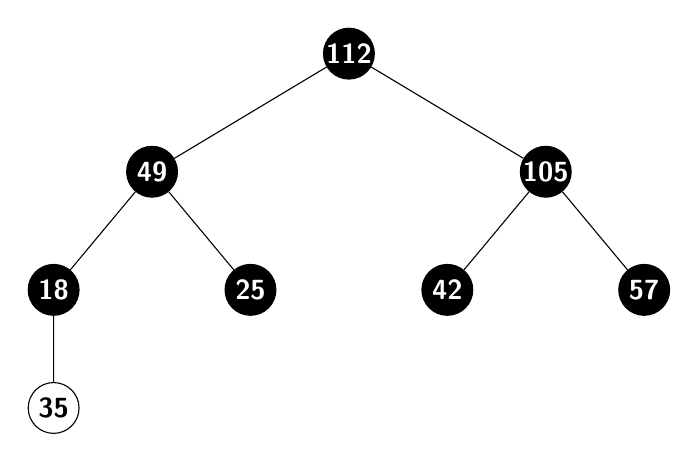
\begin{tikzpicture}[level/.style={sibling distance = 5cm/#1,
  level distance = 1.5cm}] 
  \node [arn_n] {112}
   child{ node [arn_n] {49}
    child{ node [arn_n] {18}
        child{ node [arn_t] {35}}
    }
    child{ node [arn_n] {25}}
    }
   child{ node [arn_n] {105}
    child{ node [arn_n] {42}}
    child{ node [arn_n] {57}}
   }
;
\end{tikzpicture}
\\
\\
\textbf{Adding 35 to the heap. Conflict found. Bubbling up}
\\
\\

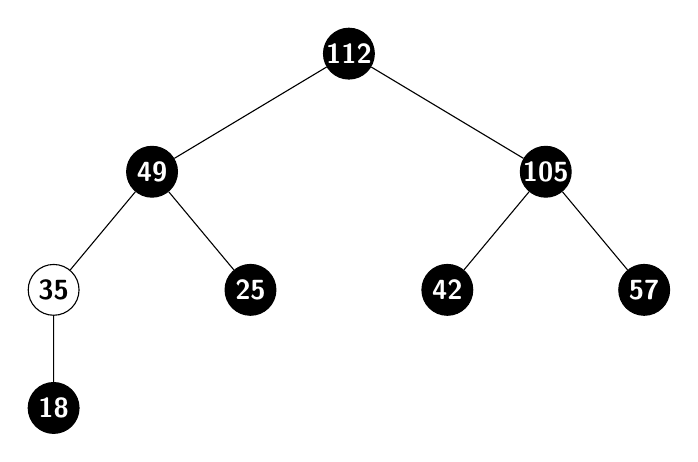
\begin{tikzpicture}[level/.style={sibling distance = 5cm/#1,
  level distance = 1.5cm}] 
  \node [arn_n] {112}
   child{ node [arn_n] {49}
    child{ node [arn_t] {35}
        child{ node [arn_n] {18}}
    }
    child{ node [arn_n] {25}}
    }
   child{ node [arn_n] {105}
    child{ node [arn_n] {42}}
    child{ node [arn_n] {57}}
   }
;
\end{tikzpicture}
\\
\\
\textbf{Swapping with its parents. $35>18$. No remaining conflict}
\\
\\

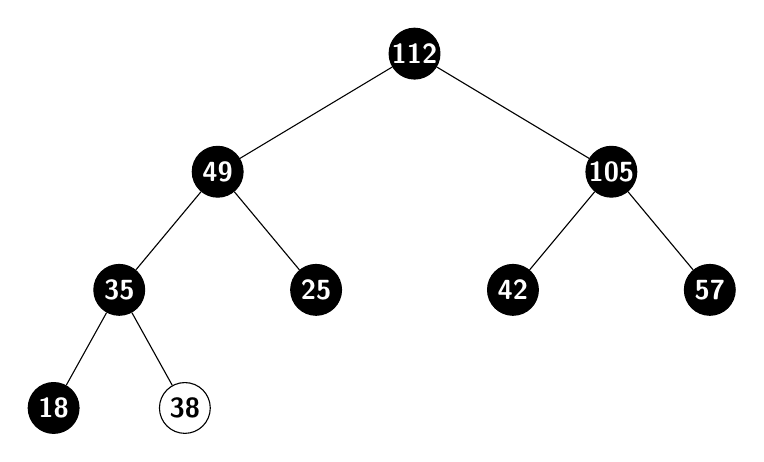
\begin{tikzpicture}[level/.style={sibling distance = 5cm/#1,
  level distance = 1.5cm}] 
  \node [arn_n] {112}
   child{ node [arn_n] {49}
    child{ node [arn_n] {35}
        child{ node [arn_n] {18}}
        child{ node [arn_t] {38}}
    }
    child{ node [arn_n] {25}}
    }
   child{ node [arn_n] {105}
    child{ node [arn_n] {42}}
    child{ node [arn_n] {57}}
   }
;
\end{tikzpicture}
\\
\\
\textbf{Adding 38 to the heap. Conflict found. Bubbling up}
\\
\\

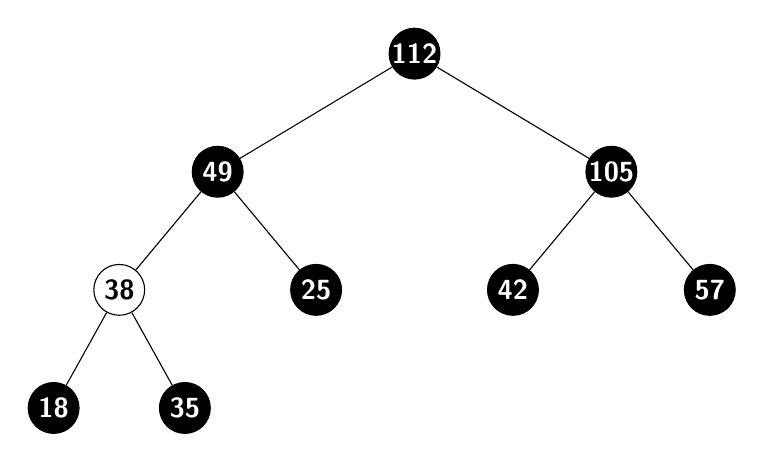
\begin{tikzpicture}[level/.style={sibling distance = 5cm/#1,
  level distance = 1.5cm}] 
  \node [arn_n] {112}
   child{ node [arn_n] {49}
    child{ node [arn_t] {38}
        child{ node [arn_n] {18}}
        child{ node [arn_n] {35}}
    }
    child{ node [arn_n] {25}}
    }
   child{ node [arn_n] {105}
    child{ node [arn_n] {42}}
    child{ node [arn_n] {57}}
   }
;
\end{tikzpicture}
\\
\\
\textbf{Swapping with its parents. $38>35$. No remaining conflict}
\\
\\

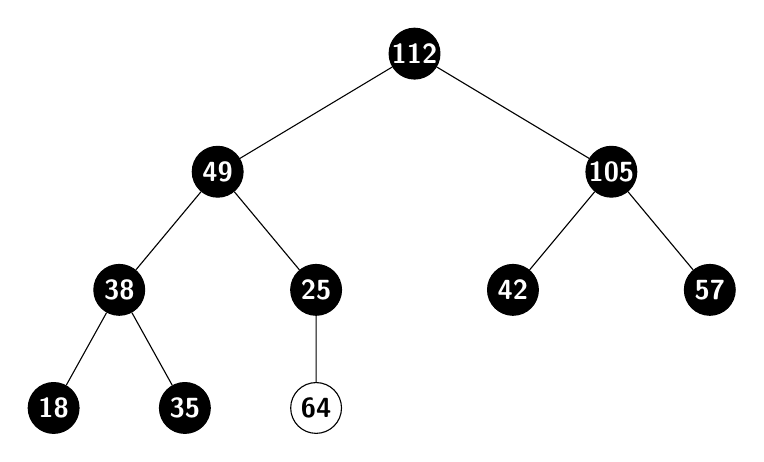
\begin{tikzpicture}[level/.style={sibling distance = 5cm/#1,
  level distance = 1.5cm}] 
  \node [arn_n] {112}
   child{ node [arn_n] {49}
    child{ node [arn_n] {38}
        child{ node [arn_n] {18}}
        child{ node [arn_n] {35}}
    }
    child{ node [arn_n] {25}
        child{ node [arn_t] {64}}
    }
    }
   child{ node [arn_n] {105}
    child{ node [arn_n] {42}}
    child{ node [arn_n] {57}}
   }
;
\end{tikzpicture}
\\
\\
\textbf{Adding 64 to the heap. Conflict found. Bubbling up}
\\
\\

\begin{tikzpicture}[level/.style={sibling distance = 5cm/#1,
  level distance = 1.5cm}] 
  \node [arn_n] {112}
   child{ node [arn_n] {49}
    child{ node [arn_n] {38}
        child{ node [arn_n] {18}}
        child{ node [arn_n] {35}}
    }
    child{ node [arn_t] {64}
        child{ node [arn_n] {25}}
    }
    }
   child{ node [arn_n] {105}
    child{ node [arn_n] {42}}
    child{ node [arn_n] {57}}
   }
;
\end{tikzpicture}
\\
\\
\textbf{Swapping with its parents. $64>25$. Still having conflict. Continue bubbling up}
\\
\\

\begin{tikzpicture}[level/.style={sibling distance = 5cm/#1,
  level distance = 1.5cm}] 
  \node [arn_n] {112}
   child{ node [arn_t] {64}
    child{ node [arn_n] {38}
        child{ node [arn_n] {18}}
        child{ node [arn_n] {35}}
    }
    child{ node [arn_n] {49}
        child{ node [arn_n] {25}}
    }
    }
   child{ node [arn_n] {105}
    child{ node [arn_n] {42}}
    child{ node [arn_n] {57}}
   }
;
\end{tikzpicture}
\\
\\
\textbf{Swapping with its parents. $64>49$. No remaining conflict}
\\
\\

\begin{tikzpicture}[level/.style={sibling distance = 5cm/#1,
  level distance = 1.5cm}] 
  \node [arn_n] {112}
   child{ node [arn_n] {64}
    child{ node [arn_n] {38}
        child{ node [arn_n] {18}}
        child{ node [arn_n] {35}}
    }
    child{ node [arn_n] {49}
        child{ node [arn_n] {25}}
        child{ node [arn_t] {53}}
    }
    }
   child{ node [arn_n] {105}
    child{ node [arn_n] {42}}
    child{ node [arn_n] {57}}
   }
;
\end{tikzpicture}
\\
\\
\textbf{Adding 53 to the heap. Conflict found. Bubbling up}
\\
\\

\begin{tikzpicture}[level/.style={sibling distance = 5cm/#1,
  level distance = 1.5cm}] 
  \node [arn_n] {112}
   child{ node [arn_n] {64}
    child{ node [arn_n] {38}
        child{ node [arn_n] {18}}
        child{ node [arn_n] {35}}
    }
    child{ node [arn_t] {53}
        child{ node [arn_n] {25}}
        child{ node [arn_n] {49}}
    }
    }
   child{ node [arn_n] {105}
    child{ node [arn_n] {42}}
    child{ node [arn_n] {57}}
   }
;
\end{tikzpicture}
\\
\\
\textbf{Swapping with its parents. $53>49$. No remaining conflict}
\\
\\

\begin{tikzpicture}[level/.style={sibling distance = 5cm/#1,
  level distance = 1.5cm}] 
  \node [arn_n] {112}
   child{ node [arn_n] {64}
    child{ node [arn_n] {38}
        child{ node [arn_n] {18}}
        child{ node [arn_n] {35}}
    }
    child{ node [arn_n] {53}
        child{ node [arn_n] {25}}
        child{ node [arn_n] {49}}
    }
    }
   child{ node [arn_n] {105}
    child{ node [arn_n] {42}
        child{ node [arn_t] {20}}
    }
    child{ node [arn_n] {57}}
   }
;
\end{tikzpicture}
\\
\\
\textbf{Adding 20 to the heap. No conflict found}
\\
\\

\begin{tikzpicture}[level/.style={sibling distance = 5cm/#1,
  level distance = 1.5cm}] 
  \node [arn_n] {112}
   child{ node [arn_n] {64}
    child{ node [arn_n] {38}
        child{ node [arn_n] {18}}
        child{ node [arn_n] {35}}
    }
    child{ node [arn_n] {53}
        child{ node [arn_n] {25}}
        child{ node [arn_n] {49}}
    }
    }
   child{ node [arn_n] {105}
    child{ node [arn_n] {42}
        child{ node [arn_n] {20}}
        child{ node [arn_t] {25}}
    }
    child{ node [arn_n] {57}}
   }
;
\end{tikzpicture}
\\
\\
\textbf{Adding 25 to the heap. No conflict found}
\\
\\

\begin{tikzpicture}[level/.style={sibling distance = 5cm/#1,
  level distance = 1.5cm}] 
  \node [arn_n] {112}
   child{ node [arn_n] {64}
    child{ node [arn_n] {38}
        child{ node [arn_n] {18}}
        child{ node [arn_n] {35}}
    }
    child{ node [arn_n] {53}
        child{ node [arn_n] {25}}
        child{ node [arn_n] {49}}
    }
    }
   child{ node [arn_n] {105}
    child{ node [arn_n] {42}
        child{ node [arn_n] {20}}
        child{ node [arn_n] {25}}
    }
    child{ node [arn_n] {57}
        child{ node [arn_t] {19}}
    }
   }
;
\end{tikzpicture}
\\
\\
\textbf{Adding 19 to the heap. No conflict found}
\\
\\

\begin{tikzpicture}[level/.style={sibling distance = 5cm/#1,
  level distance = 1.5cm}] 
  \node [arn_n] {112}
   child{ node [arn_n] {64}
    child{ node [arn_n] {38}
        child{ node [arn_n] {18}}
        child{ node [arn_n] {35}}
    }
    child{ node [arn_n] {53}
        child{ node [arn_n] {25}}
        child{ node [arn_n] {49}}
    }
    }
   child{ node [arn_n] {105}
    child{ node [arn_n] {42}
        child{ node [arn_n] {20}}
        child{ node [arn_n] {25}}
    }
    child{ node [arn_n] {57}
        child{ node [arn_n] {19}}
        child{ node [arn_t] {16}}
    }
   }
;
\end{tikzpicture}
\\
\\
\textbf{Adding 16 to the heap. No conflict found}
\\
\\
\subsection{Final Max-heap tree}
\begin{tikzpicture}[level/.style={sibling distance = 5cm/#1,
  level distance = 1.5cm}] 
  \node [arn_n] {112}
   child{ node [arn_n] {64}
    child{ node [arn_n] {38}
        child{ node [arn_n] {18}}
        child{ node [arn_n] {35}}
    }
    child{ node [arn_n] {53}
        child{ node [arn_n] {25}}
        child{ node [arn_n] {49}}
    }
    }
   child{ node [arn_n] {105}
    child{ node [arn_n] {42}
        child{ node [arn_n] {20}}
        child{ node [arn_n] {25}}
    }
    child{ node [arn_n] {57}
        child{ node [arn_n] {19}}
        child{ node [arn_n] {16}}
    }
   }
;
\end{tikzpicture} %-- done
\section{Trees}
\subsection{Instruction}

Given 2 trees T1 and T2, where T1 has more nodes than T2, and where each of the nodes in both
trees holds an integer value. Further, the values in any of the trees are assumed to be unique (no
duplicate values within the same tree).
\begin{itemize}
\item[] i) Give an algorithm that determines whether or not T2 represents a subtree of T1.
\item[] ii) What is the time and space complexity of your algorithm in i)?
\item[] iii) Will your algorithm still work if duplicate values are permitted in these trees?

\begin{itemize}
\item[] a. If your algorithm still works when duplicate values are allowed, explain clearly
why this change could not have affected your solution.
\item[] b. If your algorithm will fail if duplicate values are allowed, provide an example of
the failure and propose some modification to fix this failure. 
\end{itemize}
\end{itemize}

\subsection{Check sub-tree}


\begin{algorithm}[H]
\caption{Check if a tree is the subtree of another tree or not}
\textbf{Input:} Root node of trees t1, t2, in which t1 is the tree with the number of nodes is equal or greater than that of t2.
\\
\textbf{Output:} a boolean value indicates if t2 is a subtree of t1.
\begin{algorithmic}[1]
\Procedure{isSubTree}{TreeNode rootT1, TreeNode rootT2}
\State ArrayList t1 $\leftarrow$ null
\State ArrayList t2 $\leftarrow$ null
\State preOrder(rootT1, t1)
\State preOrder(rootT2, t2)
\State \Return isSubList(t1, t2)
\EndProcedure
\end{algorithmic}
\end{algorithm}
\textbf{Two dependent methods to support the main isSubTree method:}
\\
\\
\begin{algorithm}[H]
\caption{}
\textbf{Input:} A root node of a tree. An array list acts as a container for all the nodes inside the given tree.
\\
\textbf{Output:} Assign the given arrayList to have all the nodes in the given tree with pre order traversal. 
\begin{algorithmic}[1]
\Procedure{preOrder}{TreeNode node, ArrayList t}
\State t.add(node)
\ForEach{$\text{child } \textbf{w} \in \textbf{node}$}
\State preOrder(w)
\EndFor
\EndProcedure
\end{algorithmic}
\end{algorithm}

\begin{algorithm}[H]
\caption{}
\textbf{Input:} An array list of the tree which has the number of nodes is more or equal than that of the second array list.
\\
\textbf{Output:} A boolean value indicates if the array list t2 is a sub array of t1
\begin{algorithmic}[1]
\Procedure{isSubList}{ArrayList t1, ArrayList t2}
\State i $\leftarrow$ 0
\State j $\leftarrow$ 0

\While {i $<$ t1.size \textbf{and} j $<$ t2.size}
\If{t1[i] = t2[j]}
\State i++
\State j++

\If{j = t2.size} 
\Return true \Comment{iterated over t2.}
\EndIf

\Else
\State i++
\State j $\leftarrow$ 0
\EndIf

\EndWhile

\Return false
\EndProcedure
\end{algorithmic}
\end{algorithm}


\subsection{Time and Space complexity}
\textit{The problem concerns of 2 different input: tree 1 and tree 2. Let denote the number of nodes inside the first tree t1 to be n, and that of the second tree t2 to be m.}
\begin{itemize}
    \item \textbf{Time Complexity:} The algorithm takes n, m time for t1, t2 respectively to iterate and put every node into the 2 created array lists. Therefore, it takes \textbf{n + m} time for this operation. Next, the algorithm calls the function \textbf{isSubList} to check if one of the array list is the sub array of the other. By doing this, the algorithm has to iterate over every element in the bigger array which has n elements. Thus, the time it takes here is \textbf{n}. In conclusion, the algorithm takes up to \textbf{O(n + m)} of time complexity.
    \item \textbf{Space Complexity:} The algorithm creates 2 new array lists to hold the elements from both trees. Thus, the space needs to be allocated is the total number of elements in both tree, which is  \textbf{n + m}. Space complexity is of \textbf{O(n+m)}.
\end{itemize}

\subsection{Algorithm still works if there are duplicate values?}
The proposed algorithm above will work even when there are some duplicated elements inside one of the two given trees. Since the approach was to take all elements and put into one array list, and then check if one of them is the sub array of the other, it would guarantee that there is no possible misbehaviour with duplicated items.


 %-- done 
\section{The important of AVAILABLE object in linear probing for Hash-tables}

\subsection{Instruction}
Assume the utilization of linear probing for hash-tables. To enhance the complexity of the
operations performed on the table, a special AVAILABLE object is used. Assuming that all keys
are positive integers, the following two techniques were suggested in order to enhance complexity:
\begin{itemize}
    \item 
\item[] i) In case an entry is removed, instead of marking its location as AVAILABLE, indicate
the key as the negative value of the removed key (i.e. if the removed key was 16,
indicate the key as -16). Searching for an entry with the removed key would then
terminate once a negative value of the key is found (instead of continuing to search if
AVAILABLE is used).

\item[] ii) Instead of using AVAILABLE, find a key in the table that should have been placed in
the location of the removed entry, then place that key (place the entire entry of course)
in that location (instead of setting the location as AVAILABLE). The motive is to find
the key faster since it is now in its hashed location. This would also avoid the
dependence on the AVAILABLE object.
\end{itemize}
Will either of these proposals enhance the search time complexity? Additionally, will any of these
approaches result in misbehaviour (in terms of functionalities, or even performance)? If so, explain
clearly through illustrative examples. 

\subsection{Claim:}
\textbf{In this particular problem, since the statement indicates the sign of interchange in keywords "key" and "hash-value", the answer for this also assumes the interchanging of these two keywords. However, the distinction in the keywords is still important to be recognized in order to avoid any further confusion. "Key" is usually referred to an entry in a pair of element (key, value), while "hash-value" is usually the integer value of a key after being hashed by a function. In this problem, to whom read this, please perceive the term "key" as in fact, "hash value". }

\subsection{Consider alternative method I}
The first proposal will not change the \textit{search} time complexity at all since the algorithm still has to iterate through all the probes, and eventually reaches the \textbf{recent removed entry} with negative value. Thus, the time complexity for \textit{search} operation is still \textbf{O(n)}, which means it does not improve anything.
\\
Moreover, there is a high chance the algorithm will \textbf{misbehaviour} in many situations. 
\\
\textbf{Consider the following situation:}
\\
\begin{tikzpicture}
    [%%%%%%%%%%%%%%%%%%%%%%%%%%%%%%
        box/.style={rectangle,draw=black, ultra thick, minimum size=1cm},
    ]%%%%%%%%%%%%%%%%%%%%%%%%%%%%%%
\foreach \x/\y in {0/\text{$\dots$},1/16,2/16,3/16,4/16,5/16,6/\text{$\dots$}}
        \node[box] at (\x,0){\y};

\draw[decorate,decoration={brace,mirror},thick] (0.7,-.7) -- node[below]{Probes of key 16} (5.5,-.7);
\draw[->,very thick] (1,1.2) --  node[above,yshift=2mm]{i} (1,.7);

\end{tikzpicture}
\\
\textbf{Remove A[i]. Then as proposed, replace the key with negative value.}
\\
\begin{tikzpicture}
    [%%%%%%%%%%%%%%%%%%%%%%%%%%%%%%
        box/.style={rectangle,draw=black, ultra thick, minimum size=1cm},
    ]%%%%%%%%%%%%%%%%%%%%%%%%%%%%%%
\foreach \x/\y in {0/\text{$\dots$},1/-16,2/16,3/16,4/16,5/16,6/\text{$\dots$}}
        \node[box] at (\x,0){\y};

\draw[decorate,decoration={brace,mirror},thick] (0.7,-.7) -- node[below]{Probes of key 16} (5.5,-.7);
\draw[->,very thick] (1,1.2) --  node[above,yshift=2mm]{i} (1,.7);

\end{tikzpicture}
\\
In this situation, when using \textit{search} algorithm for key 16, the algorithm will stop at A[i], and return null indicating there is no such key in the array. While in reality, there are plenty of entries with key 16 in the probes after -16. Therefore, the algorithm misses the actual results.
\\
In fact, the algorithm only behaves as expected when there is \textbf{only} one single probe of a key. If that is the case, then it completely defeats the purpose of open-addressing.

\subsection{Consider alternative method II}
This proposed method will make a slightly improvement in \textit{search} operation in the hash-table. However, it may lead to a more serious problem in term of algorithm behaviour. For example:
\\
\begin{tikzpicture}
    [%%%%%%%%%%%%%%%%%%%%%%%%%%%%%%
        box/.style={rectangle,draw=black, ultra thick, minimum size=1cm},
    ]%%%%%%%%%%%%%%%%%%%%%%%%%%%%%%
\foreach \x/\y in {0/\text{$\dots$},1/16,2/16,3/16,4/16,5/16,6/\text{$\dots$}}
        \node[box] at (\x,0){\y};

\draw[decorate,decoration={brace,mirror},thick] (0.7,-.7) -- node[below]{Probes of key 16} (5.5,-.7);
\draw[->,very thick] (1,1.2) --  node[above,yshift=2mm]{i} (1,.7);
\draw[->,very thick] (2,1.2) --  node[above,yshift=2mm]{j} (2,.7);

\end{tikzpicture}
\\
\textbf{Removing the first element in the probe. Then found another key to replace the removed position}
\\
\begin{tikzpicture}
    [%%%%%%%%%%%%%%%%%%%%%%%%%%%%%%
        box/.style={rectangle,draw=black, ultra thick, minimum size=1cm},
    ]%%%%%%%%%%%%%%%%%%%%%%%%%%%%%%
\foreach \x/\y in {0/\text{$\dots$},1/16,2/,3/16,4/16,5/16,6/\text{$\dots$}}
        \node[box] at (\x,0){\y};

\draw[decorate,decoration={brace,mirror},thick] (0.7,-.7) -- node[below]{Probes of key 16} (5.5,-.7);
\draw[->,very thick] (1,1.2) --  node[above,yshift=2mm]{i} (1,.7);
\draw[->,very thick] (2,1.2) --  node[above,yshift=2mm]{j} (2,.7);
\end{tikzpicture}
\\
The \textit{search} operation will terminate at A[j] since it is an empty position (indicating the end of probe). But in fact, there are more elements with the same key after that empty position. Thus, the algorithm misses checking those elements, resulting in a possible lost of searching results. 
\\
However, this problem could be avoided if the algorithm was implemented by checking every position after the first-found possible hashed location. But this results in a time complexity of \textit{O(n)}, which means it does not improve anything. As a matter of fact, the algorithm is even slower in some cases than that using AVAILABLE object. Implementing the mechanism of AVAILABLE object will provide a chance to terminate the algorithm by reaching empty position without having to iterate until the last element in the table.



 %-- done 
\section{Collision handling with separate chaining}
\subsection{Instruction}
Assume a hash table utilizes an array of 13 elements and that collisions are handled by separate
chaining. Considering the hash function is defined as: h(k)=k mod 13.
\begin{itemize}
\item i) Draw the contents of the table after inserting elements with the following keys:
\begin{center}
\text{32, 147, 265, 195, 207, 180, 21, 16, 189, 202, 91, 94, 162, 75, 37, 77, 81, 48}
\end{center}
\item ii) What is the maximum number of collisions caused by the above insertions?
\end{itemize}

\subsection{Contents of the Hash-table}
\begin{tikzpicture}
\coordinate (0);
\foreach \t[count=\i from 0,evaluate=\i as\j using int(\i+1)] in {
195 $\rightarrow$ 91  ,
null,
null,
16  $\rightarrow$ 94 $\rightarrow$ 81  ,
147 ,
265 ,
32  $\rightarrow$ 162 ,
189 ,
21  $\rightarrow$ 202 ,
48  ,
10  ,
180 $\rightarrow$ 37  ,
207 $\rightarrow$ 77  
}
\node at(\i.south)[anchor=north,draw,minimum height=2em,minimum width=1.5em,outer sep=0pt](\j){}
    node at(\j.west)[align=right,left]{\i} 
    node at(\j.east)[align=left,right,xshift=-.7em]{$\rightarrow$ \t};
\end{tikzpicture}
\\
\textbf{Contents of the Hash-table after inserting}

\subsection{Maximum number of collisions}
The maximum number of collisions is 3 collisions, happened at index 3 of the table with 3 values 16, 94, 81. The maxim %-- done
\section{Attempt to reduce collisions in separate chaining}
\subsection{Instruction}
To reduce the maximum number of collisions in the hash table described in Question 7 above,
someone proposed the use of a larger array of 15 elements (that is roughly 15\% bigger) and of
course modifying the hash function to: h(k)=k mod 15. The idea is to reduce the load factor and
hence the number of collisions.
\\
\\
Does this proposal hold any validity to it? If yes, indicate why such modifications would actually
reduce the number of collisions. If no, indicate clearly the reasons you believe/think that such
proposal is senseless. 

\subsection{Use a larger array to achieve a better load factor}
The idea of reducing load factor by increasing the size of an array is actually a good solution to lower the number of collisions. When the size of the table is expanded, the distribution of hash value could be more uniformly, and well distributed. In another word, the probability of getting an uniformed distribution increases. Thus, a better load factor could be achieved. 
\\
However, with such a small increase with a small set of number as in the current case (expand from 13 elements to 15 elements), the improvement will just be a slight change. The number of collisions even could stay the same despite the decrease of the load factor.  %-- done
\section{Double-Hashing for collision handling}
\subsection{Instruction}
Assume an open addressing hash table implementation, where the size of the array is N = 19,
and that \textit{double hashing} is performed for collision handling. The second hash function is defined
as:
\begin{center}
\textbf{d(k) = q - k mod q}
\end{center}
where k is the key being inserted in the table and the prime number q is = 7. Use simple modular
operation (k mod N) for the first hash function. 
\begin{itemize}
    \item i) Show the content of the table after performing the following operations, in order:
    \textbf{put(25), put(12), put(42), put(31), put(35), put(39), remove(31), put(48),
    remove(25), put(18), put(29), put(29), put(35).}
    \item ii) What is the size of the longest cluster caused by the above insertions?
    \item iii) What is the number of occurred collisions as a result of the above operations?
    \item iv) What is the current value of the table’s \textit{load factor}?
    \\
\end{itemize}

\textbf{Summary}
\begin{itemize} 
    \item q = 7
    \item N = 19
    \item 1st hash function: \textbf{k mod N}
    \item 2nd hash function: \textbf{d(k) = q - k mod q}
\end{itemize}

\subsection{Contents of the hash-table}
\begin{center}
 \begin{tabular}{||c c c c c||} 
 \hline
 Operation & k & h(k) & d(k) & Probes \\ [2ex] 
 \hline \hline
 \textbf{put} & 25 & 6 & 3 & 6 \\
 \textbf{put} & 12 & 12 & 2 & 12 \\
 \textbf{put} & 42 & 4 & 7 & 4 \\
 \textbf{put} & 31 & 12 & 4 & 12 $\rightarrow$ 16 \\
 \textbf{put} & 35 & 16 & 7 & 16 $\rightarrow$ 4 $\rightarrow$ 11 \\ 
 \textbf{put} & 39 & 1 & 3 & 1 \\
 \textbf{remove} & 31 & $\emptyset$ & $\emptyset$ & AVAILABLE object at 16 \\
 \textbf{put} & 48 & 10 & 1 & 10 \\
 \textbf{remove} & 25 & $\emptyset$ & $\emptyset$ & AVAILABLE object at 6 \\
 \textbf{put} & 18 & 18 & 3 & 18 \\
 \textbf{put} & 29 & 10 & 6 & 10 $\rightarrow$ 16 \\
 \textbf{put} & 29 & 10 & 6 & 10 $\rightarrow$ 16 $\rightarrow$ 3 \\
 \textbf{put} & 35 & 16 & 7 & 16 $\rightarrow$ 4 $\rightarrow$ 11 $\rightarrow$ 18 $\rightarrow$ 6 \\ [2ex]
 \hline 
 \end{tabular}
 \\
 \textbf{Table to construct the hash table}
\end{center}

\begin{tikzpicture}
\coordinate (0);
\foreach \t[count=\i from 0,evaluate=\i as\j using int(\i+1)] in {
null,
39,
null,
29,
42,
null,
35,
null,
null,
null,
48,
35,
12,
null,
null,
null,
29,
null,
18
}
\node at(\i.south)[anchor=north,draw,minimum height=2em,minimum width=1.5em,outer sep=0pt](\j){}
    node at(\j.west)[align=right,left]{\i} 
    node at(\j.east)[align=left,right,xshift=-.7em]{$\rightarrow$ \t};
\end{tikzpicture}
\\
\textbf{Hash Table}
\\

\subsection{Size of the longest cluster}
The longest cluster has size of 3 at index 10, 11, and 12 consecutively.

\subsection{Number of occured collisions}
There were 10 collisions happened.

\subsection{Current load factor}
\begin{itemize}
    \item The table is an array of size 19 $\rightarrow$ N = 19
    \item Currently, there are 9 elements inside the hash table $\rightarrow$ n = 9
\end{itemize}
$\rightarrow$ \textit{The load factor = } $\frac{n}{N} = \frac{9}{19} \approx 0.47$ %-- done 
\section{Radix-sort}
\subsection{Instruction}
Show the steps that a radix sort takes when sorting the following array of integer keys:
\begin{center}
\textbf{832 91 411 172 243 573 326 292 682 489 96}
\end{center}

\subsection{Run Radix-Sort through the array}
\textbf{The original array}
\\
\\
\begin{tikzpicture}
        [box/.style={rectangle,draw=black, ultra thick, minimum size=1cm},]
\foreach \x/\y in {0/832, 1/91, 2/411, 3/172, 4/243, 5/573, 6/326, 7/292, 8/682, 9/489, 10/96}
        \node[box] at (\x,0){\y};
\end{tikzpicture}
\\
\\
\textbf{Run the first round of radix-sort with the most right bit of each key}
\\
\\
\begin{tikzpicture}
        [box/.style={rectangle,draw=black, ultra thick, minimum size=1cm},]
\foreach \x/\y in {0/83\ul{2}, 1/9\ul{1}, 2/41\ul{1}, 3/17\ul{2}, 4/24\ul{3}, 5/57\ul{3}, 6/32\ul{6}, 7/29\ul{2}, 8/68\ul{2}, 9/48\ul{9}, 10/9\ul{6}}
        \node[box] at (\x,0){\y};
\end{tikzpicture}
\\
\\
\textbf{Result as: }
\\
\\
\begin{tikzpicture}
        [box/.style={rectangle,draw=black, ultra thick, minimum size=1cm},]
\foreach \x/\y in {0/91, 1/411, 2/832, 3/172, 4/292, 5/682, 6/243, 7/573, 8/326, 9/96, 10/489}
        \node[box] at (\x,0){\y};
\end{tikzpicture}
\\
\\
\textbf{Run the second round with the second bit}
\\
\\
\begin{tikzpicture}
        [box/.style={rectangle,draw=black, ultra thick, minimum size=1cm},]
\foreach \x/\y in {0/\ul{9}1, 1/4\ul{1}1, 2/8\ul{3}2, 3/1\ul{7}2, 4/2\ul{9}2, 5/6\ul{8}2, 6/2\ul{4}3, 7/5\ul{7}3, 8/3\ul{2}6, 9/\ul{9}6, 10/4\ul{8}9}
        \node[box] at (\x,0){\y};
\end{tikzpicture}
\\
\\
\textbf{Result as: }
\\
\\
\begin{tikzpicture}
        [box/.style={rectangle,draw=black, ultra thick, minimum size=1cm},]
\foreach \x/\y in {0/411, 1/326, 2/832, 3/243, 4/172, 5/573, 6/682, 7/489, 8/91, 9/292, 10/96}
        \node[box] at (\x,0){\y};
\end{tikzpicture}
\\
\\
\textbf{Run the third round with the third bit}
\\
\\
\begin{tikzpicture}
        [box/.style={rectangle,draw=black, ultra thick, minimum size=1cm},]
\foreach \x/\y in {0/\ul{4}11, 1/\ul{3}26, 2/\ul{8}32, 3/\ul{2}43, 4/\ul{1}72, 5/\ul{5}73, 6/\ul{6}82, 7/\ul{4}89, 8/\ul{0}91, 9/\ul{2}92, 10/\ul{0}96}
        \node[box] at (\x,0){\y};
\end{tikzpicture}
\\
\\
\textbf{Result as: }
\\
\\
\begin{tikzpicture}
        [box/.style={rectangle,draw=black, ultra thick, minimum size=1cm},]
\foreach \x/\y in {0/91, 1/96, 2/172, 3/243, 4/292, 5/326, 6/411, 7/489, 8/573, 9/682, 10/832}
        \node[box] at (\x,0){\y};
\end{tikzpicture}
\\
\\
\textbf{The maximum length of a key is 3. The algorithm has gone through 3 rounds $\rightarrow$ Terminate radix-sort. The array  of integer keys was sorted.} %-- done
\section{AVL tree}
\begin{tikzpicture}[level/.style={sibling distance = 70mm/#1,
  level distance = 1cm}] 
  \node [arn_n] {55}
    child{ node [arn_n] {29}
        child{node [arn_n] {17}
            child{node [arn_x] {}}
            child{node [arn_x] {}}
        }
        child{node [arn_n] {44}
            child{node [arn_n] {35}
                child{node [arn_x] {}}
                child{node [arn_x] {}}
            }
            child{node [arn_x] {}}
        }
   }
    child{ node [arn_n] {84}
        child{ node [arn_n] {62}
            child{ node [arn_n] {2}
                child{node [arn_x] {}}
                child{node [arn_x] {}}
            }
            child{ node [arn_n] {82}
                child{ node [arn_n] {75}
                    child{node [arn_x] {}}
                    child{node [arn_n] {81}
                        child{node [arn_x] {}}
                        child{node [arn_x] {}}
                        }
                }
                child{node [arn_x] {}}
            }
        }
        child{ node [arn_n] {93}
            child{ node [arn_n] {89}
                child{node [arn_x] {}}
                child{node [arn_x] {}}
            }
            child{node [arn_x] {}}
        }
    }
;
\end{tikzpicture}

\subsection{Instruction}
\begin{itemize}
    \item 
Are there any errors with the tree as shown? If so, indicate what the error(s) are, correct
these error(s) [you should attempt applying the smallest possible number of changes to
correct the tree], show the corrected AVL tree, then proceed to the following questions
(Questions ii to iv) and start with the tree that you have just corrected. If no errors are
there in the above tree, indicate why the tree is correctly an AVL tree, then proceed to
the following questions (Questions ii to iv) and continue working on the tree as shown
above.
\item ii) Show the AVL tree after put(74) operation is performed. Give the complexity of this
operation in terms of Big-O notation.
\item iii) Show the AVL tree after remove(62) is performed. Give the complexity of this
operation in terms of Big-O notation.
\item iv) Show the AVL tree after remove(93) is performed. Show the progress of your work
step-by-step. Give the complexity of this operation in terms of Big-O notation.
\end{itemize}


\subsection{Check errors with the given AVL tree}
\textit{The error lying at the subtree of 82. The right sub tree has height 0 while the left subtree has heigh of 2. Thus, it is a violation of AVL tree's property.}
\\
\\
\begin{tikzpicture}[level/.style={sibling distance = 70mm/#1,
  level distance = 1cm}] 
  \node [arn_n] {55}
    child{ node [arn_n] {29}
        child{node [arn_n] {17}
            child{node [arn_x] {}}
            child{node [arn_x] {}}
        }
        child{node [arn_n] {44}
            child{node [arn_n] {35}
                child{node [arn_x] {}}
                child{node [arn_x] {}}
            }
            child{node [arn_x] {}}
        }
   }
    child{ node [arn_n] {84}
        child{ node [arn_n] {62}
            child{ node [arn_n] {2}
                child{node [arn_x] {}}
                child{node [arn_x] {}}
            }
            child{ node [arn_o] {82}
                child{ node [arn_o] {75}
                    child{node [arn_x] {}}
                    child{node [arn_o] {81}
                        child{node [arn_x] {}}
                        child{node [arn_x] {}}
                        }
                }
                child{node [arn_x] {}}
            }
        }
        child{ node [arn_n] {93}
            child{ node [arn_n] {89}
                child{node [arn_x] {}}
                child{node [arn_x] {}}
            }
            child{node [arn_x] {}}
        }
    }
;
\end{tikzpicture}
\\
\\
\textbf{After restructuring the sub tree of 82}
\\
\\
\begin{tikzpicture}[level/.style={sibling distance = 70mm/#1,
  level distance = 1cm}] 
  \node [arn_n] {55}
    child{ node [arn_n] {29}
        child{node [arn_n] {17}
            child{node [arn_x] {}}
            child{node [arn_x] {}}
        }
        child{node [arn_n] {44}
            child{node [arn_n] {35}
                child{node [arn_x] {}}
                child{node [arn_x] {}}
            }
            child{node [arn_x] {}}
        }
   }
    child{ node [arn_n] {84}
        child{ node [arn_n] {62}
            child{ node [arn_n] {2}
                child{node [arn_x] {}}
                child{node [arn_x] {}}
            }
            child{ node [arn_t] {81}
                child{ node [arn_t] {75}
                    child{node [arn_x] {}}
                    child{node [arn_x] {}}
                }
                child{ node [arn_t] {82}
                    child{node [arn_x] {}}
                    child{node [arn_x] {}}
                }
            }
        }
        child{ node [arn_n] {93}
            child{ node [arn_n] {89}
                child{node [arn_x] {}}
                child{node [arn_x] {}}
            }
            child{node [arn_x] {}}
        }
    }
;
\end{tikzpicture}
\\
\\
\textbf{Final result:}
\\
\\
\begin{tikzpicture}[level/.style={sibling distance = 70mm/#1,
  level distance = 1cm}] 
  \node [arn_n] {55}
    child{ node [arn_n] {29}
        child{node [arn_n] {17}
            child{node [arn_x] {}}
            child{node [arn_x] {}}
        }
        child{node [arn_n] {44}
            child{node [arn_n] {35}
                child{node [arn_x] {}}
                child{node [arn_x] {}}
            }
            child{node [arn_x] {}}
        }
   }
    child{ node [arn_n] {84}
        child{ node [arn_n] {62}
            child{ node [arn_n] {2}
                child{node [arn_x] {}}
                child{node [arn_x] {}}
            }
            child{ node [arn_n] {81}
                child{ node [arn_n] {75}
                    child{node [arn_x] {}}
                    child{node [arn_x] {}}
                }
                child{ node [arn_n] {82}
                    child{node [arn_x] {}}
                    child{node [arn_x] {}}
                }
            }
        }
        child{ node [arn_n] {93}
            child{ node [arn_n] {89}
                child{node [arn_x] {}}
                child{node [arn_x] {}}
            }
            child{node [arn_x] {}}
        }
    }
;
\end{tikzpicture}

\subsection{Put(74)}
\subsubsection{Perform the operation}

\begin{tikzpicture}[level/.style={sibling distance = 70mm/#1,
  level distance = 1cm}] 
  \node [arn_n] {55}
    child{ node [arn_n] {29}
        child{node [arn_n] {17}
            child{node [arn_x] {}}
            child{node [arn_x] {}}
        }
        child{node [arn_n] {44}
            child{node [arn_n] {35}
                child{node [arn_x] {}}
                child{node [arn_x] {}}
            }
            child{node [arn_x] {}}
        }
   }
    child{ node [arn_n] {84}
        child{ node [arn_n] {62}
            child{ node [arn_n] {2}
                child{node [arn_x] {}}
                child{node [arn_x] {}}
            }
            child{ node [arn_n] {81}
                child{ node [arn_n] {75}
                    child{node [arn_o] {74}
                        child{node [arn_x] {}}
                        child{node [arn_x] {}}
                    }
                    child{node [arn_x] {}}
                }
                child{ node [arn_n] {82}
                    child{node [arn_x] {}}
                    child{node [arn_x] {}}
                }
            }
        }
        child{ node [arn_n] {93}
            child{ node [arn_n] {89}
                child{node [arn_x] {}}
                child{node [arn_x] {}}
            }
            child{node [arn_x] {}}
        }
    }
;
\end{tikzpicture}
\\
\\
\textbf{Need restructuring at the subtree of 62.}
\\
\\
\begin{tikzpicture}[level/.style={sibling distance = 70mm/#1,
  level distance = 1cm}] 
  \node [arn_n] {55}
    child{ node [arn_n] {29}
        child{node [arn_n] {17}
            child{node [arn_x] {}}
            child{node [arn_x] {}}
        }
        child{node [arn_n] {44}
            child{node [arn_n] {35}
                child{node [arn_x] {}}
                child{node [arn_x] {}}
            }
            child{node [arn_x] {}}
        }
   }
    child{ node [arn_n] {84}
        child{ node [arn_o] {62}
            child{ node [arn_n] {2}
                child{node [arn_x] {}}
                child{node [arn_x] {}}
            }
            child{ node [arn_o] {81}
                child{ node [arn_o] {75}
                    child{node [arn_t] {74}
                        child{node [arn_x] {}}
                        child{node [arn_x] {}}
                    }
                    child{node [arn_x] {}}
                }
                child{ node [arn_n] {82}
                    child{node [arn_x] {}}
                    child{node [arn_x] {}}
                }
            }
        }
        child{ node [arn_n] {93}
            child{ node [arn_n] {89}
                child{node [arn_x] {}}
                child{node [arn_x] {}}
            }
            child{node [arn_x] {}}
        }
    }
;
\end{tikzpicture}
\\
\\
\textbf{After restructuring:}
\\
\\
\begin{tikzpicture}[level/.style={sibling distance = 70mm/#1,
  level distance = 1cm}] 
  \node [arn_n] {55}
    child{ node [arn_n] {29}
        child{node [arn_n] {17}
            child{node [arn_x] {}}
            child{node [arn_x] {}}
        }
        child{node [arn_n] {44}
            child{node [arn_n] {35}
                child{node [arn_x] {}}
                child{node [arn_x] {}}
            }
            child{node [arn_x] {}}
        }
   }
    child{ node [arn_n] {84}
        child{ node [arn_t] {75}
            child{ node [arn_t] {62}
                child{ node [arn_n] {2}
                    child{node [arn_x] {}}
                    child{node [arn_x] {}}
                }
                child{ node [arn_n] {74}
                    child{node [arn_x] {}}
                    child{node [arn_x] {}}
                }
            }
            child{ node [arn_t] {81}
                child{node [arn_x] {}}
                child{ node [arn_n] {82}
                    child{node [arn_x] {}}
                    child{node [arn_x] {}}
                }
            }
        }
        child{ node [arn_n] {93}
            child{ node [arn_n] {89}
                child{node [arn_x] {}}
                child{node [arn_x] {}}
            }
            child{node [arn_x] {}}
        }
    }
;
\end{tikzpicture}
\\
\\
\textbf{Final result:}
\\
\\
\begin{tikzpicture}[level/.style={sibling distance = 70mm/#1,
  level distance = 1cm}] 
  \node [arn_n] {55}
    child{ node [arn_n] {29}
        child{node [arn_n] {17}
            child{node [arn_x] {}}
            child{node [arn_x] {}}
        }
        child{node [arn_n] {44}
            child{node [arn_n] {35}
                child{node [arn_x] {}}
                child{node [arn_x] {}}
            }
            child{node [arn_x] {}}
        }
   }
    child{ node [arn_n] {84}
        child{ node [arn_n] {75}
            child{ node [arn_n] {62}
                child{ node [arn_n] {2}
                    child{node [arn_x] {}}
                    child{node [arn_x] {}}
                }
                child{ node [arn_n] {74}
                    child{node [arn_x] {}}
                    child{node [arn_x] {}}
                }
            }
            child{ node [arn_n] {81}
                child{node [arn_x] {}}
                child{ node [arn_n] {82}
                    child{node [arn_x] {}}
                    child{node [arn_x] {}}
                }
            }
        }
        child{ node [arn_n] {93}
            child{ node [arn_n] {89}
                child{node [arn_x] {}}
                child{node [arn_x] {}}
            }
            child{node [arn_x] {}}
        }
    }
;
\end{tikzpicture}


\subsubsection{Time complexity}
To find the place to put a new node at the beginning, it takes n time. In addition, to find out if there is a need for restructuring, the algorithm has to run log n time. To actually restructure the tree to suit the AVL tree's property, it takes constant time, meaning 1 in Big-O. In conclusion, the whole operation has the time complexity of \textbf{O(logn).}

\subsection{remove(62)}
\subsubsection{Perform the operation}
\textbf{Final result:}
\\
\\
\begin{tikzpicture}[level/.style={sibling distance = 70mm/#1,
  level distance = 1cm}] 
  \node [arn_n] {55}
    child{ node [arn_n] {29}
        child{node [arn_n] {17}
            child{node [arn_x] {}}
            child{node [arn_x] {}}
        }
        child{node [arn_n] {44}
            child{node [arn_n] {35}
                child{node [arn_x] {}}
                child{node [arn_x] {}}
            }
            child{node [arn_x] {}}
        }
   }
    child{ node [arn_n] {84}
        child{ node [arn_n] {75}
            child{ node [arn_n] {74}
                child{ node [arn_n] {2}
                    child{ node [arn_x] {}}
                    child{ node [arn_x] {}}
                }
                child{ node [arn_x] {}}
            } 
            child{ node [arn_n] {81}
                child{node [arn_x] {}}
                child{ node [arn_n] {82}
                    child{node [arn_x] {}}
                    child{node [arn_x] {}}
                }
            }
        }
        child{ node [arn_n] {93}
            child{ node [arn_n] {89}
                child{node [arn_x] {}}
                child{node [arn_x] {}}
            }
            child{node [arn_x] {}}
        }
    }
;
\end{tikzpicture}

\subsubsection{Time complexity}
The time complexity is \textbf{O(log n)} since the algorithm has to find where to remove (log n), and then check if it needs restructuring or not (takes log n).

\subsection{remove(93)}
\subsubsection{Step-by-step progress}
\textbf{Remove(93). Traverse to find the replace node for 93. Found 89}
\\
\\
\begin{tikzpicture}[level/.style={sibling distance = 70mm/#1,
  level distance = 1cm}] 
  \node [arn_n] {55}
    child{ node [arn_n] {29}
        child{node [arn_n] {17}
            child{node [arn_x] {}}
            child{node [arn_x] {}}
        }
        child{node [arn_n] {44}
            child{node [arn_n] {35}
                child{node [arn_x] {}}
                child{node [arn_x] {}}
            }
            child{node [arn_x] {}}
        }
   }
    child{ node [arn_n] {84}
        child{ node [arn_n] {75}
            child{ node [arn_n] {74}
                child{ node [arn_n] {2}
                    child{ node [arn_x] {}}
                    child{ node [arn_x] {}}
                }
                child{ node [arn_x] {}}
            } 
            child{ node [arn_n] {81}
                child{node [arn_x] {}}
                child{ node [arn_n] {82}
                    child{node [arn_x] {}}
                    child{node [arn_x] {}}
                }
            }
        }
        child{ node [arn_o] {93}
            child{ node [arn_o] {89}
                child{node [arn_x] {}}
                child{node [arn_x] {}}
            }
            child{node [arn_x] {}}
        }
    }
;
\end{tikzpicture}
\\
\\
\textbf{Remove 93. Replace 93 by 89}
\\
\\
\begin{tikzpicture}[level/.style={sibling distance = 70mm/#1,
  level distance = 1cm}] 
  \node [arn_n] {55}
    child{ node [arn_n] {29}
        child{node [arn_n] {17}
            child{node [arn_x] {}}
            child{node [arn_x] {}}
        }
        child{node [arn_n] {44}
            child{node [arn_n] {35}
                child{node [arn_x] {}}
                child{node [arn_x] {}}
            }
            child{node [arn_x] {}}
        }
   }
    child{ node [arn_n] {84}
        child{ node [arn_n] {75}
            child{ node [arn_n] {74}
                child{ node [arn_n] {2}
                    child{ node [arn_x] {}}
                    child{ node [arn_x] {}}
                }
                child{ node [arn_x] {}}
            } 
            child{ node [arn_n] {81}
                child{node [arn_x] {}}
                child{ node [arn_n] {82}
                    child{node [arn_x] {}}
                    child{node [arn_x] {}}
                }
            }
        }
        child{ node [arn_o] {89}
            child{node [arn_x] {}}
            child{node [arn_x] {}}
        }
    }
;
\end{tikzpicture}
\\
\\
\textbf{Need to restructure. The subtree 84 is violating AVL tree's property.}
\\
\\
\begin{tikzpicture}[level/.style={sibling distance = 70mm/#1,
  level distance = 1cm}] 
  \node [arn_n] {55}
    child{ node [arn_n] {29}
        child{node [arn_n] {17}
            child{node [arn_x] {}}
            child{node [arn_x] {}}
        }
        child{node [arn_n] {44}
            child{node [arn_n] {35}
                child{node [arn_x] {}}
                child{node [arn_x] {}}
            }
            child{node [arn_x] {}}
        }
   }
    child{ node [arn_o] {84}
        child{ node [arn_o] {75}
            child{ node [arn_o] {74}
                child{ node [arn_n] {2}
                    child{ node [arn_x] {}}
                    child{ node [arn_x] {}}
                }
                child{ node [arn_x] {}}
            } 
            child{ node [arn_n] {81}
                child{node [arn_x] {}}
                child{ node [arn_n] {82}
                    child{node [arn_x] {}}
                    child{node [arn_x] {}}
                }
            }
        }
        child{ node [arn_n] {89}
            child{node [arn_x] {}}
            child{node [arn_x] {}}
        }
    }
;
\end{tikzpicture}
\\
\\
\textbf{Use 3 main nodes: 84, 75, 74 to restructure the sub tree. Resulting:}
\\
\\
\begin{tikzpicture}[level/.style={sibling distance = 70mm/#1,
  level distance = 1cm}] 
  \node [arn_n] {55}
    child{ node [arn_n] {29}
        child{node [arn_n] {17}
            child{node [arn_x] {}}
            child{node [arn_x] {}}
        }
        child{node [arn_n] {44}
            child{node [arn_n] {35}
                child{node [arn_x] {}}
                child{node [arn_x] {}}
            }
            child{node [arn_x] {}}
        }
   }
   child{ node [arn_n] {75}
        child{ node [arn_n] {74}
            child{ node [arn_n] {2}
                child{ node [arn_x] {}}
                child{ node [arn_x] {}}
            }    
            child{ node [arn_x] {}}
        }
        child{ node [arn_n] {84}
           child{ node [arn_n] {81}
                child{ node [arn_x] {}}
                child{ node [arn_n] {82}
                    child{ node [arn_x] {}}
                    child{ node [arn_x] {}}
                } 
           } 
           child{ node [arn_n] {89}
                child{ node [arn_x] {}}
                child{ node [arn_x] {}}
           }
        }
   }
;
\end{tikzpicture}

\subsubsection{Time complexity}
In order to find the node to replace 93, the algorithm has to traverse log n time to find 93 and log n time to find the element that can replace the position of 93. Then, the algorithm has to run log n time to restructuring the tree. In conclusion, the total operation has time complexity of \textbf{O(log n).}















 %-- done

\end{document}